\chapter{Results of the cross-section measurement}
\minitoc

In this chapter results of the W/Z cross-section measurements will be discussed. 
In Sec. \ref{sec:flavCs} the cross-sections measured in each lepton flavors are presented. These results are used to test lepton universality in 2.76 TeV data.

Section \ref{sec:CombCs} describes a results obtained for combined W and Z cross-sections. Additionally, in the subsection the cross-section ratios are presented. In the final section, the interpretation of the results using the the PDF profiling method is presented.

\section{Cross-sections results}\label{sec:flavCs}

The cross-sections are calculated separately for each boson and lepton flavor as described in Chap.~\ref{chap:Met}. The sources of uncertainties on the measurements are discussed in Chap.~\ref{chap:Unc}. Table \ref{tab:Wcs} summarizes the obtained $W^{+/-}$ and Z cross-sections obtained from 2.76 TeV data in fiducial and extrapolated full and 13 TeV regions. The uncertainty coming from luminosity (labeled lumi) is a dominant one for this measurement. The statistical uncertainty is labeled stat. and is the second dominant uncertainty for the W and Z bosons cross-section. For W boson in electron channel the systematic uncertainty is around 1\%, that makes it significantly lower, than a statistical uncertainty. For W boson in a muon channel cross-sections the overall systematical uncertainty is higher because of the trigger scale factors, and is around 1.2\%, that makes it comparable with the statistical uncertainty.  The results are consistent between lepton flavors. 

%\begin{table}[!tbp]
\begin{center}
\caption{Number of observed candidates N and expected background events B, efficiency, acceptance and extrapolation correction factors for the W and Z bosons in electron and muon channels. Monte Carlo corrections are included in the $C_{W/Z}$ factors. The given uncertainties are the quadratic sum of statistical and systematic components.}
\label{tab:Values}
\begin{tabular}{l | c c c c }
\hline
\hline
 & $N_{W/Z}^{sig}$ & $C_{W/Z}$ & $A_{W/Z}$ & $E_{W/Z}$ \\
 \hline
& \multicolumn{4}{c}{Electron channel}\\
 \hline
 $W^{+}\to e\nu$  & & & & \\
 $W^{-}\to e\nu$ & & & & \\
 $Z \to ee$ & & & & \\
 \hline
 & \multicolumn{4}{c}{Muon channel} \\
  \hline
  $W^{+}\to \mu\nu$  & & & & \\
 $W^{-}\to \mu\nu$ & & & & \\
 $Z \to \mu \mu $ & & & & \\
 \hline
\end{tabular}
\end{center}
\end{table}

\begin{table}[!tb]
\caption{Results on a fiducial $\sigma^{fid}$ and total cross-section measurement for $W^{+}$, $W^{-}$ and Z bosons in electron and muon channels. The cross-sections are shown with their statistical, systematical and luminosity uncertainties (and extrapolation error for total cross-section) quoted in that order}
\label{tab:Wcs}
\begin{center}
\begin{tabular}{| l | c | c |}
\hline
 & value $\pm$ stat $\pm$ syst $\pm$ lumi ($\pm$ ext)& value $\pm$ stat $\pm$ syst $\pm$ lumi ($\pm$ ext) \\
 \hline
 \hline
 & \multicolumn{2}{c|}{W in electron channel}\\
& $W^{+}\to e\nu$ & $W^{-}\to e\nu$ \\

\hline
$\sigma^{fid}_{W}$ [pb]  & \sigfidWplusenunolabel & \sigfidWminenunolabel \\
$\sigma^{tot}_{W}$ [pb] & \sigtotWplusenunolabel & \sigtotWminenunolabel \\
$\sigma^{13}_{W}$ [pb] & \sigTrWplusenunolabel & \sigTrWminenunolabel \\
\hline
\hline
 & \multicolumn{2}{c|}{W in muon channel}\\
& $W^{+}\to \mu\nu$ & $W^{-}\to \mu\nu$\\
\hline
$\sigma^{fid}_{W}$ [pb] & \sigfidWplusmununolabel & \sigfidWminmununolabel \\
$\sigma^{tot}_{W}$ [pb]  & \sigtotWplusmununolabel & \sigtotWminmununolabel \\
$\sigma^{13}_{W}$ [pb]  & \sigTrWplusmununolabel & \sigTrWminmununolabel \\
\hline
%\hline
 %& \multicolumn{2}{c|}{$W^{+-}$ } \\
%& $W \to e\nu$ & $W \to \mu \nu$ \\
%\hline
%$\sigma^{fid}_{W}$ &  & \\
%$\sigma^{tot}_{W}$ & & \\
%$\sigma^{13}_{W}$ & & \\
%\hline
\hline
 & \multicolumn{2}{c|}{Z} \\
& $Z \to ee$ & $ Z \to \mu\mu$ \\
\hline
$\sigma^{fid}_{Z}$  [pb] &\sigfidZeenolabel &  \sigfidZmumunolabel \\
$\sigma^{tot}_{Z}$  [pb] & \sigtotZeenolabel & \sigtotZmumunolabel \\
$\sigma^{13}_{Z}$ [pb]  & \sigTrZeenolabel & \sigTrZmumunolabel \\
\hline
\end{tabular}
\end{center}
\end{table}

\subsection{Lepton universality test}\label{sec:LeptUnivers}

\begin{figure}[!tb]
\begin{center}
\begin{minipage}[h]{0.8\linewidth}
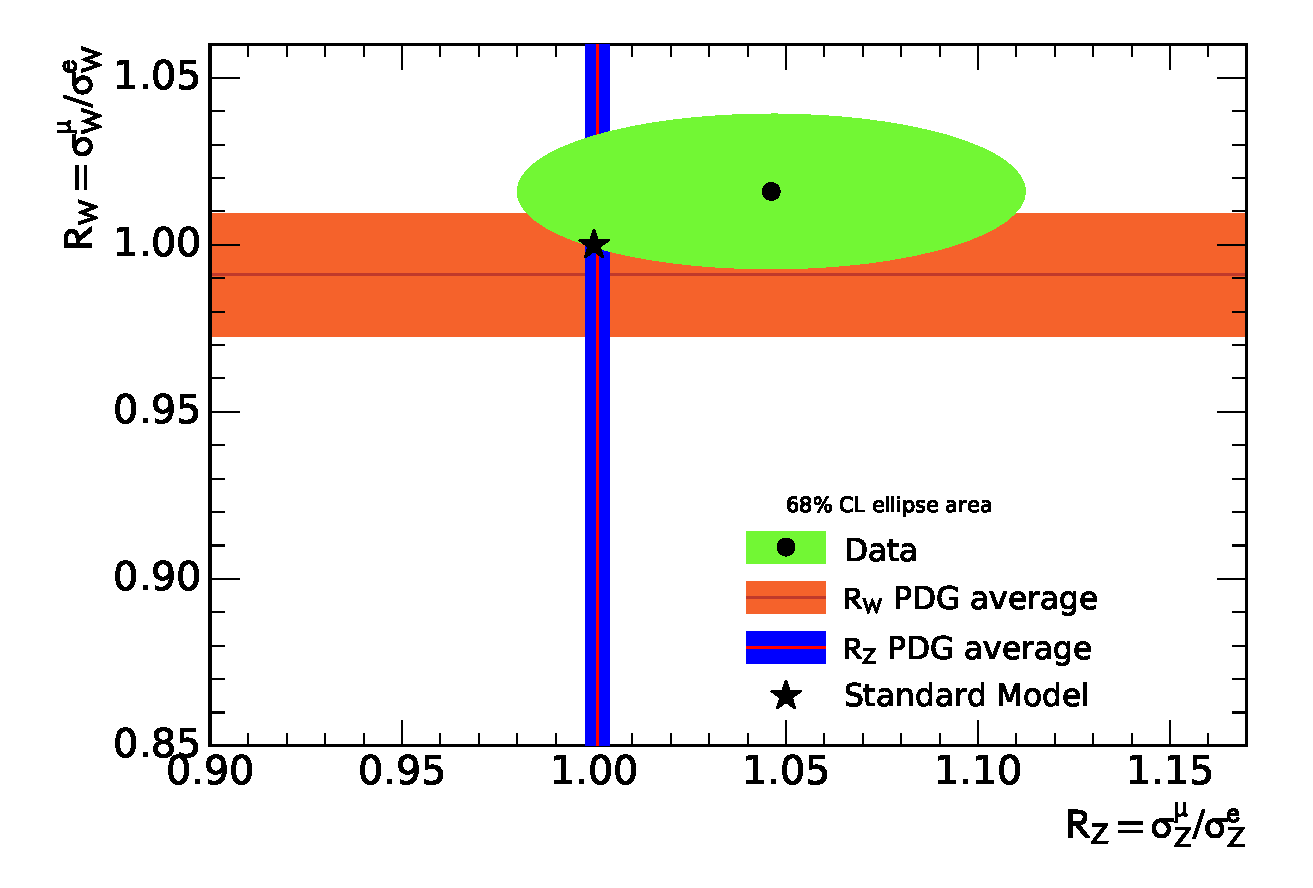
\includegraphics[width=1\textwidth]{Results/Univers.pdf}
\end{minipage}
\caption{The correlated measurement of the electron-to-muon fiducial cross-section ratios in the W and the Z channels. The vertical (horizontal) band represents the uncertainty of the cor- responding Z (W) branching fractions based on the current world average data. The green ellipse illustrates the 68\% CL for the correlated measurement of $R_W$ and $R_Z$.}
\label{fig:LeptUnivers}
\end{center}
\end{figure}


Because of the lepton universality of the Standard Model, the results, obtained in electron and muon channel are expected to agree with each other. The 2.76 TeV data could be used to test it via fiducial cross-section ratios of e and $\mu$ branching fractions:
\begin{center}
$R_{W}=\frac{\sigma^{\mu}_W}{\sigma^{e}_W} = \frac{BR(\wmunu)}{BR(\wenu)}= \valWunivers \pm \sysWunivers (sys.) \pm \statWunivers (stat.)$,
\end{center}
where the W cross-sections are calculated in fiducial region following the prescription from Sec. \ref{sec:Wcs}:
\begin{center}
$\sigma^{fid}_{W}(\wenu) = \valWenu  \pm \statWenu (stat.) \pm \sysWenu (sys.) \pm \lumiWenu (lumi.) \, [pb]$\\
$\sigma^{fid}_{W}(\wmunu) = \valWmunu  \pm \statWmunu (stat.) \pm \sysWmunu (sys.) \pm \lumiWmunu (lumi.) \, [pb]$
\end{center}
This result agrees within the uncertainty with the world average of $0.991\pm0.018$ \cite{Agashe:2014kda}. 

Similarly, this ratio can be measured in a Z boson decays as:
\begin{center}
$R_{Z}=\frac{\sigma^{\mu}_Z}{\sigma^{e}_Z} = \frac{BR(Z\to \mu\mu)}{BR(Z \to ee)}= \valZunivers \pm \sysZunivers(sys.) \pm \statZunivers (stat.)$
\end{center}
This ratio value is statistics dominated. The world average for a corresponding value is a $1.0009 \pm 0.0028$ \cite{Agashe:2014kda}. 

Comparison of the $R_W$ and $R_Z$ with the respect of the correlated systematic uncertainties with the world average is shown in Fig. \ref{fig:LeptUnivers}. The correlation matrix for $R_W$ and $R_Z$ could be found in appendix. The ellipse angle is obtained from the correlation matrix using the eigenvector decomposition and corresponds to the angle between x axis and the one of the 2 eigenvectors. The obtained values are agreeing withing the systematic uncertainty with the standard model expectations and world averages.




\section{Combined results}\label{sec:CombCs}

Since the results between channels are agreeing well, it is possible to perform averaging as described in Sec. \ref{sec:Aver}. The combination is done for fiducial region, and then combined cross-sections are extrapolated to the full and new 13 TeV regions. Systematic uncertainties for the averaging are taken from Chap. \ref{chap:Unc} with the respect of correlated uncertainties. The common luminosity uncertainty is excluded from the combination process.

\begin{table}[!tb]
\caption{Results on a fiducial $\sigma^{fid}$ and total cross-section measurement for $W^{+}$, $W^{-}$ and Z bosons in electron and muon channels. The cross-sections are shown with their statistical, systematical and luminosity uncertainties (and extrapolation error for total cross-section) quoted in that order}
\label{tab:csComb}
\begin{center}
\begin{tabular}{| l | c | c |}
\hline
 & value $\pm$ stat $\pm$ syst $\pm$ lumi ($\pm$ ext)& value $\pm$ stat $\pm$ syst $\pm$ lumi ($\pm$ ext) \\
 \hline
 \hline
 & \multicolumn{2}{c|}{$W^{+/-}$}\\
& $W^{+}\to l\nu$ & $W^{-}\to l\nu$ \\

\hline
$\sigma^{fid}_{W}$ [pb]  & $\valfidWp \pm \statfidWp \pm \sysfidWp \pm \lumifidWp$ & $\valfidWm \pm \statfidWm \pm \sysfidWm \pm \lumifidWm$ \\
$\sigma^{tot}_{W}$ [pb] & $\valfullWp \pm \statfullWp \pm \sysfullWp \pm \lumifullWp \pm \extrfullWp$ & $\valfullWm \pm \statfullWm \pm \sysfullWm \pm \lumifullWm \pm \extrfullWm$ \\
$\sigma^{13}_{W}$ [pb] & $\valthrWp \pm \statthrWp \pm \systhrWp \pm \lumithrWp$ & $\valthrWm \pm \statthrWm \pm \systhrWm \pm \lumithrWm$ \\
\hline
\hline
& \multicolumn{2}{c|}{$W \to l \nu$} \\
\hline
$\sigma^{fid}_{W}$ [pb] & \multicolumn{2}{c|}{$\valfidWtot \pm \statfidWtot \pm \sysfidWtot \pm \lumifidWtot$} \\
$\sigma^{tot}_{W}$ [pb]  & \multicolumn{2}{c|}{$\valfullWtot \pm \statfullWtot \pm \sysfullWtot \pm \lumifullWtot \pm \extrfullWtot$} \\
$\sigma^{13}_{W}$ [pb]  & \multicolumn{2}{c|}{$\valthrWtot \pm \statthrWtot \pm \systhrWtot \pm \lumithrWtot$} \\
\hline
%\hline
 %& \multicolumn{2}{c|}{$W^{+-}$ } \\
%& $W \to e\nu$ & $W \to \mu \nu$ \\
%\hline
%$\sigma^{fid}_{W}$ &  & \\
%$\sigma^{tot}_{W}$ & & \\
%$\sigma^{13}_{W}$ & & \\
%\hline
\hline
 & \multicolumn{2}{c|}{$Z \to ll$} \\
\hline
$\sigma^{fid}_{Z}$ [pb] & \multicolumn{2}{c|}{$\valfidZ \pm \statfidZ \pm \sysfidZ \pm \lumifidZ$} \\
$\sigma^{tot}_{Z}$ [pb]  & \multicolumn{2}{c|}{$\valfullZ \pm \statfullZ \pm \sysfullZ \pm \lumifullZ \pm \extrfullZ$} \\
$\sigma^{13}_{Z}$ [pb]  & \multicolumn{2}{c|}{$\valthrZ \pm \statthrZ \pm \systhrZ \pm \lumithrZ$} \\
\hline
\end{tabular}
\end{center}
\end{table}

The resulting cross-sections are summarized in Tab. \ref{tab:csComb}.  The combination procedure allows to significantly reduce statistical uncertainty of the measurement compared to the separate cross-sections. The systematic uncertainty is also visibly reduced, because most of the sources are uncorrelated for different flavors of the analysis. The combination yields a good $\chi^2/NDF\, \approx$ 1/3 indicating good agreement between measurements.  The W cross-section is calculated from the combined $W^+$ and $W^-$ cross-sections and is also in a good agreement with separate channels (Fig.~\ref{fig:Z} b).

The theoretical predictions are obtained at NLO and NNLO level of precision.  The NLO calculations are performed using the MCFM generator\cite{MCFM}, interfaced for a faster calculation with APPLGRID\cite{APPLGRID}, that provides a $x$ vs $Q^2$ grid for a calculation and convolution with the given PDF set. The NNLO predictions have been provided from the FEWZ  program \cite{FEWZ}.

The comparison of NLO and NNLO predictions for CT14nnlo\cite{CT14} pdf set for the cross-sections in fiducial region with the experimental data for separate lepton and combined channels are shown in Fig.~\ref{fig:WpNNLO} and Fig.~\ref{fig:Z}. The NLO and NNLO cross-sections are agreeing with each other and experimental data withing the PDF uncertainty. The NLO cross-sections are visibly smaller, than the obtained experimental results and have a higher uncertainty. The NNLO predictions have better agreement and a similar uncertainty.

Additionally, the obtained $W^+$, $W^-$ and $Z$ cross-sections in a combined channel are compared to the NNLO predictions for a following PDF sets: ABM12nlo\cite{ABM12}, CT14nnlo\cite{CT14}, MMHTnnlo\cite{MMHT}, ATLASepWZ12\cite{ATLASEP}, NNPDF3.0\cite{NNPDF23} and HERApdf2.0nnlo\cite{HERAPDF} in Fig.~\ref{fig:NNLODifPDFWP}-\ref{fig:NNLODifPDFZ}. The best overall agreement is achieved in a NNPDF3.0 pdf set.  Additional NNLO comparisons for full and 13 TeV regions could be found in the appendix.

\begin{figure}[!tbp]
\begin{minipage}[h]{0.45\linewidth}
\center{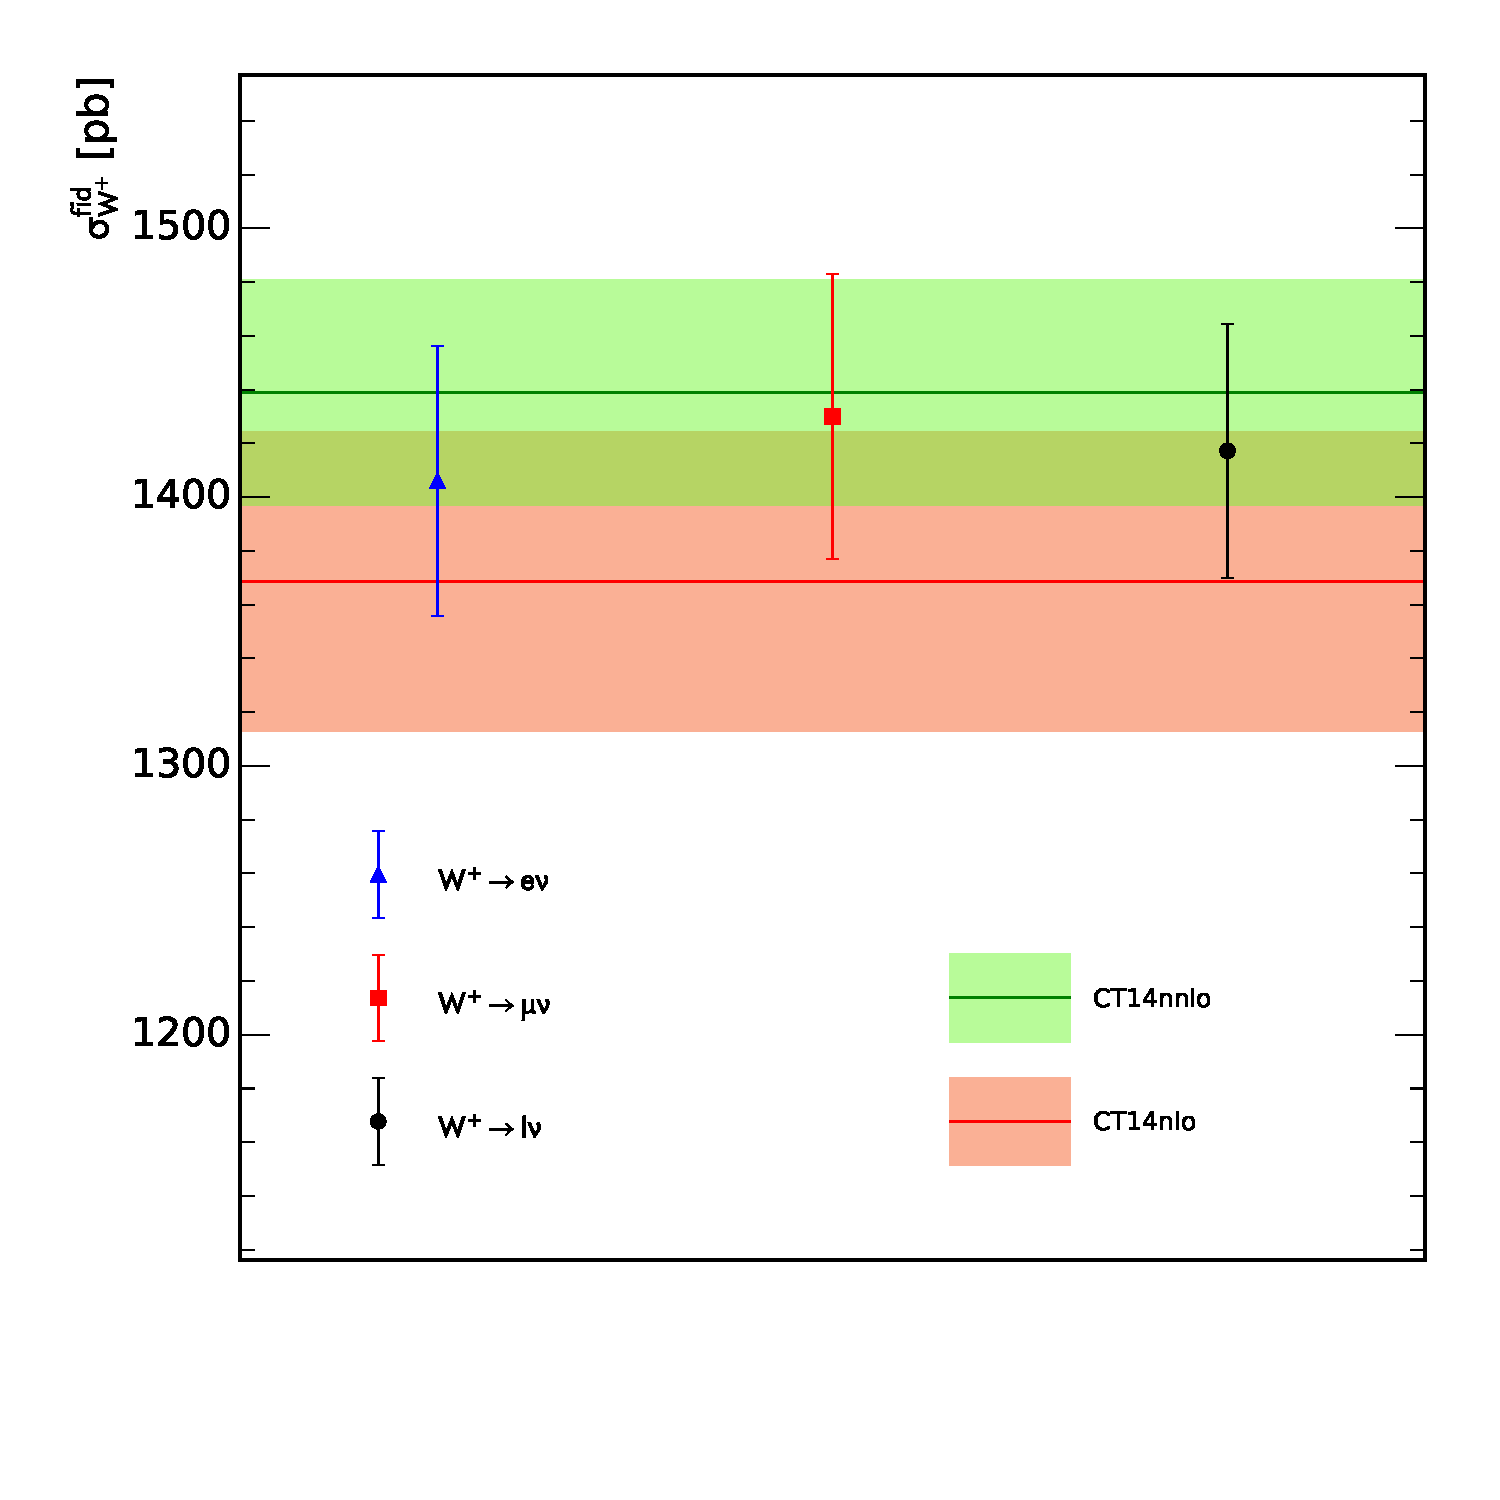
\includegraphics[width=1\textwidth]{Results/NNLOCompWPlus.pdf} \\ a)}
\end{minipage}
\hfill
\begin{minipage}[h]{0.45\linewidth}
\center{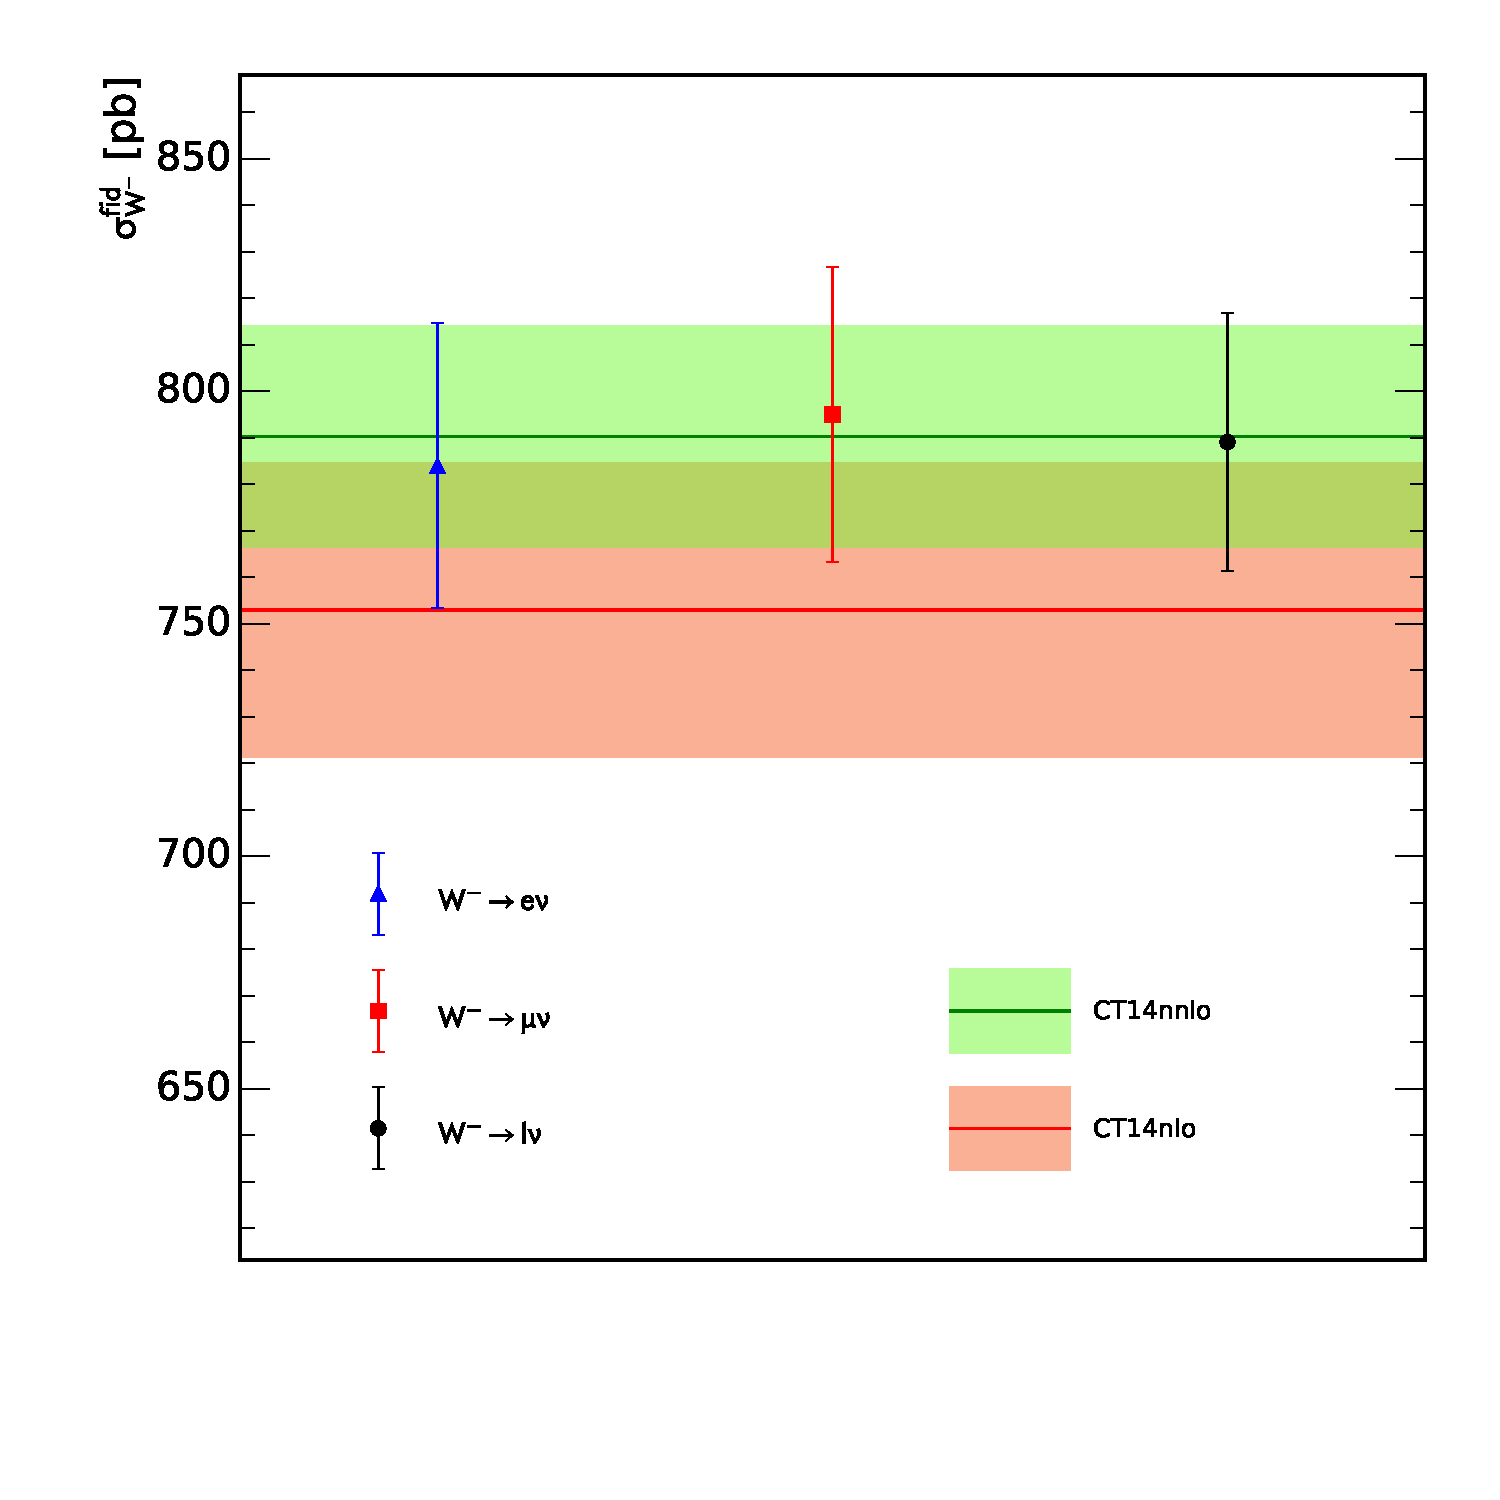
\includegraphics[width=1\textwidth]{Results/NNLOCompWMinus.pdf}\\ b)}
\end{minipage}
\caption{The NLO and NNLO theoretical predictions calculated using the CT14nnlo PDF set compared to the measured fiducial cross-sections as given in Tab.~\ref{tab:Wcs} and Tab.~\ref{tab:csComb} for a) $\sigma^{fid}_{W^{+}}$ and b) $\sigma^{fid}_{W^-}$. The blue and red dots are corresponding to the electron and muon channels respectivelly, while black dots are representing the combined channel. The NLO and NNLO predictions are presented by the red and green lines with error-bands respectively. }
\label{fig:WpNNLO}
\end{figure}

\begin{figure}[!tbp]
\begin{minipage}[h]{0.45\linewidth}
\center{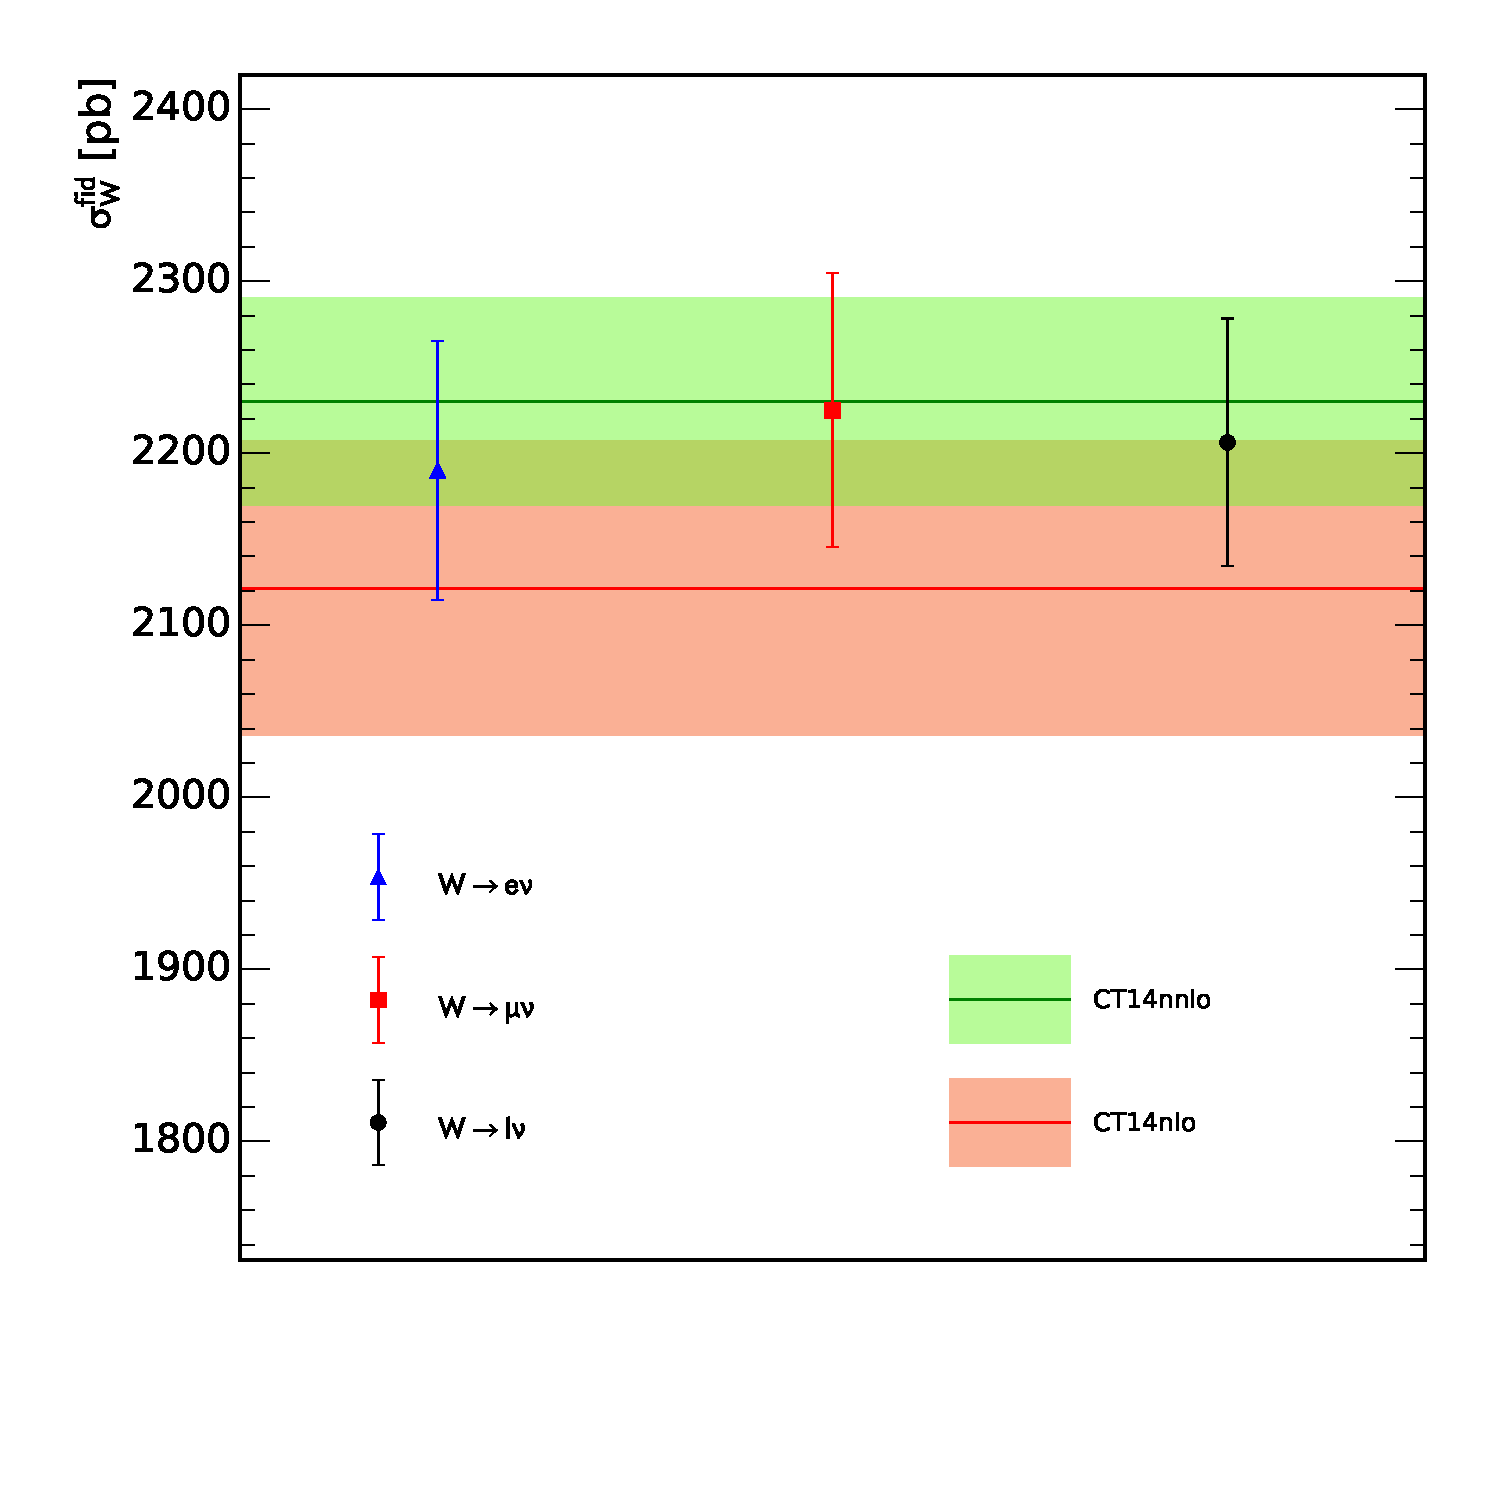
\includegraphics[width=1\textwidth]{Results/NNLOCompW.pdf} \\ a)}
\end{minipage}
\hfill
\begin{minipage}[h]{0.45\linewidth}
\center{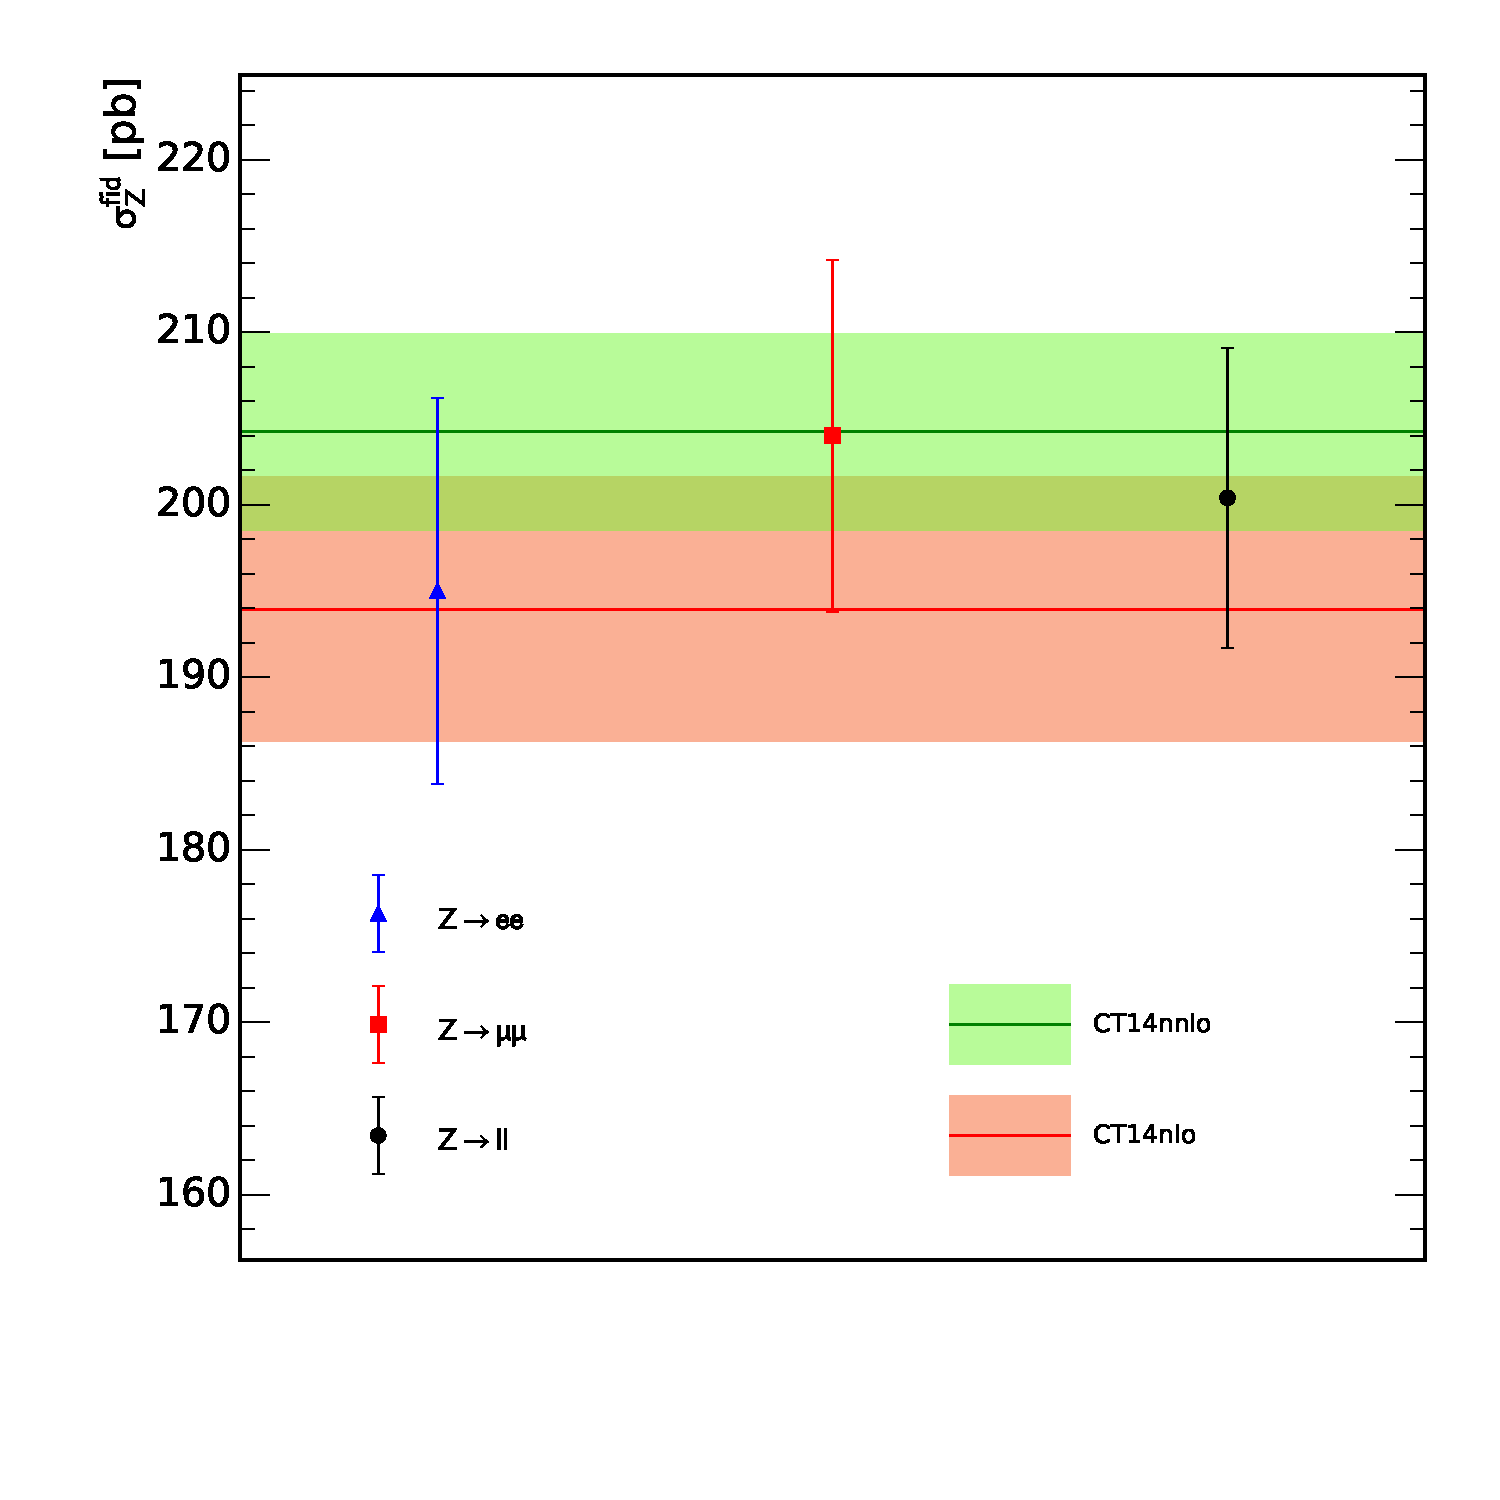
\includegraphics[width=1\textwidth]{Results/NNLOCompZ.pdf} \\ b)}
\end{minipage}
\caption{The NLO and NNLO theoretical predictions calculated using the CT14nnlo PDF set compared to the measured fiducial cross-sections as given in Tab.~\ref{tab:Wcs} and Tab.~\ref{tab:csComb} for a) $\sigma^{fid}_W$ and b) $\sigma^{fid}_Z$. The blue and red dots are corresponding to the electron and muon channels respectivelly, while black dots are representing the combined channel. The NLO and NNLO predictions are presented by the red and green lines with error-bands respectively.}
\label{fig:Z}
\end{figure}

\begin{figure}[!tbp]
\begin{center}
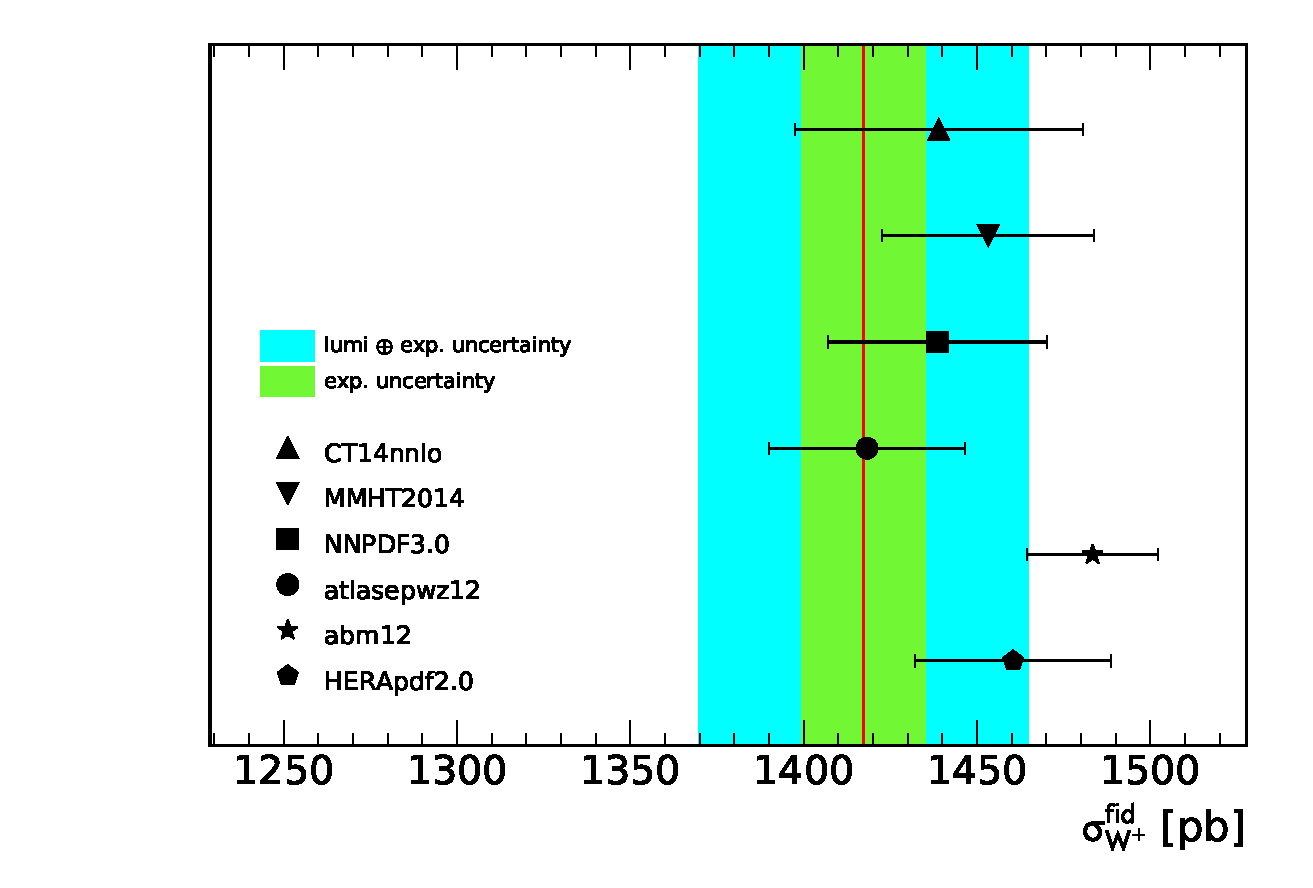
\includegraphics[width=0.7\textwidth]{Results/NNLOWPlus.pdf}
\end{center}
\caption{ NNLO predictions for the fiducial cross-section $\sigma^{fid}_{W^{+}}$ in pb for the six PDFs CT14nnlo, MMHT2014, NNPDF3.0, ATLASepWZ12, abm12, HERApdf2.0 compared to the measured fiducial cross-section as given in Tab.~\ref{tab:csComb}. The green (cyan) band corresponds to the experimental uncertainty without (with) the luminosity uncertainty. The theory predictions are given with the corresponding PDF uncertainties shown as error bands. }
\label{fig:NNLODifPDFWP}
\end{figure}

\begin{figure}[!tbp]
\begin{center}
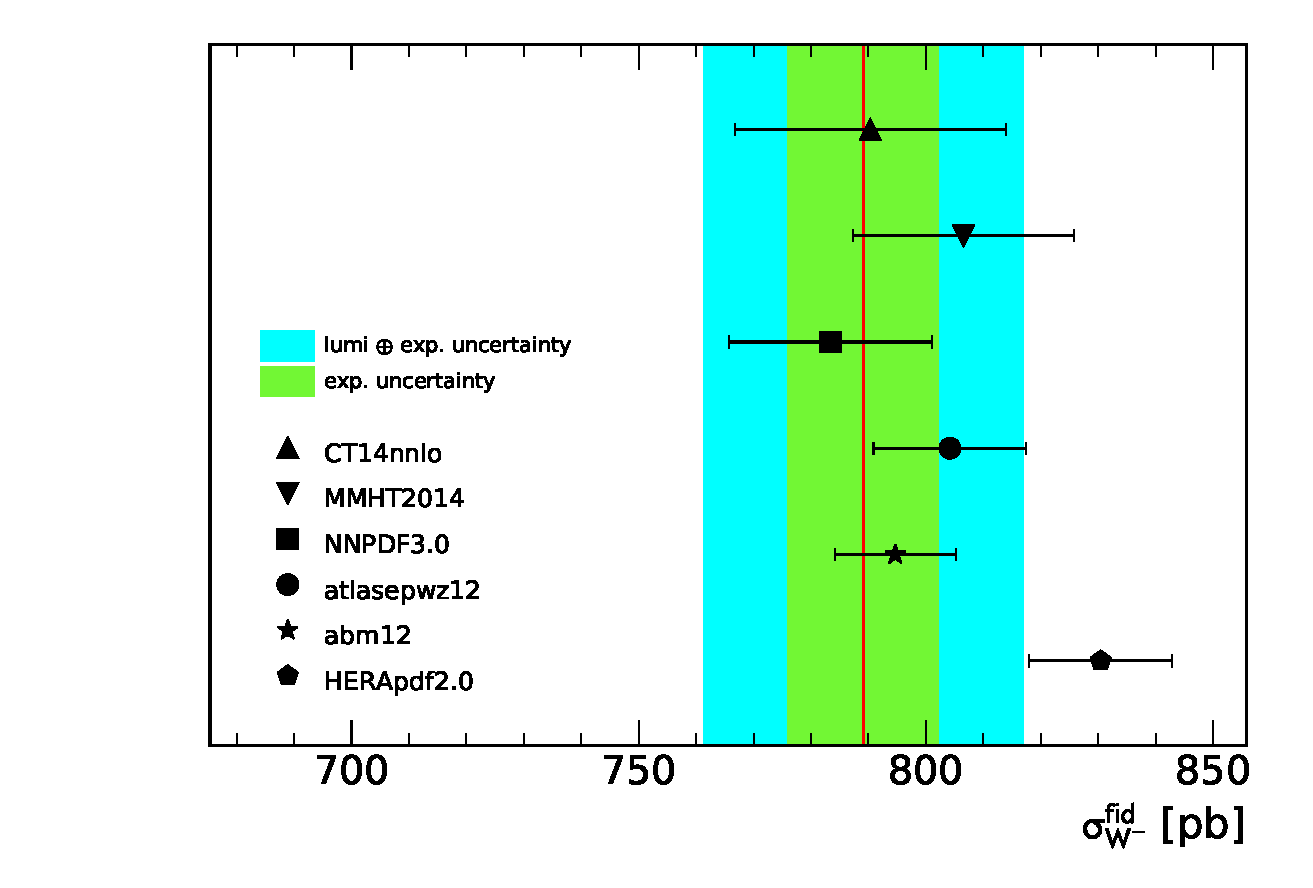
\includegraphics[width=0.7\textwidth]{Results/NNLOWMinus.pdf}
\end{center}
\caption{NNLO predictions for the fiducial cross-section $\sigma^{fid}_{W^{-}}$ in pb for the six PDFs CT14nnlo, MMHT2014, NNPDF3.0, ATLASepWZ12, abm12, HERApdf2.0 compared to the measured fiducial cross-section as given in Tab.~\ref{tab:csComb}. The green (cyan) band corresponds to the experimental uncertainty without (with) the luminosity uncertainty. The theory predictions are given with the corresponding PDF uncertainties shown as error bands.}
\label{fig:NNLODifPDFWm}
\end{figure}

\begin{figure}[!tbp]
\begin{center}
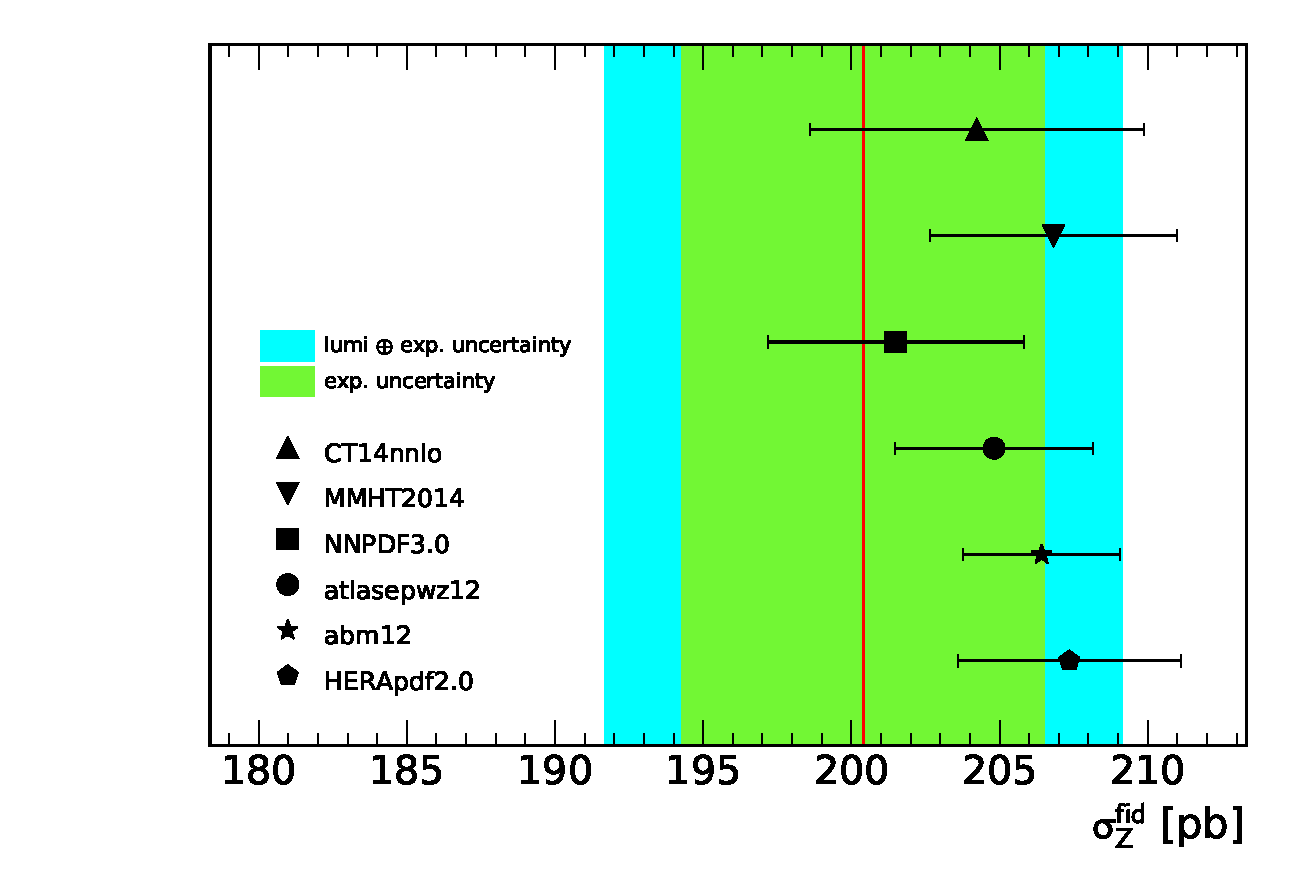
\includegraphics[width=0.7\textwidth]{Results/NNLOZ.pdf}
\end{center}
\caption{Predictions for the fiducial cross-section $\sigma^{fid}_Z$ in pb for the six PDFs CT14nnlo, MMHT2014, NNPDF3.0, ATLASepWZ12, abm12, HERApdf2.0 compared to the measured fiducial cross-section as given in Tab.~\ref{tab:csComb}. The green (cyan) band corresponds to the experimental uncertainty without (with) the luminosity uncertainty. The theory predictions are given with the corresponding PDF uncertainties shown as error bands.}
\label{fig:NNLODifPDFZ}
\end{figure}



\subsection{Cross-sections ratios}

Measurement of the ratios is a powerful tool to test PDF predictions, since it allows to cancel the biggest uncertainty coming from luminosity and reduce other sources of systematic uncertainties. The ratios of W and Z cross-sections have been measured for 7 TeV\cite{a7TeV} and 13 TeV\cite{a13TeV} analyses. The measurement of the ratio $R_{W^{+}/W^{-}}$ is sensitive to the $u_{v}$, $d_{v}$ valence quarks distributions, while the ratio $R_{W/Z}$ can put a constrains on the strange quark distributions. The ratios for W/Z cross section have been calculated in a fiducial region following the prescription from Sec.~\ref{sec:Rat} for the electron channel analyses:
\begin{center}
$R^{e}_{W/Z} = \valAelecWZ \pm \statAelecWZ \, (stat.)\, \pm \sysAelecWZ\, (sys.)\,  $ \\
$R^{e}_{W^{+}/Z} = \valAelecWpZ \pm \statAelecWpZ\, (stat.)\, \pm \sysAelecWpZ \, (sys.)\, $ \\
$R^{e}_{W^{-}/Z} = \valAelecWmZ \pm \statAelecWmZ\, (stat.)\,  \pm \sysAelecWmZ\,  (sys.)\, $ \\
$R^{e}_{W^{+}/W^{-}} = \valAelecWpWm \pm \statAelecWpWm\, (stat.)\, \pm \sysAelecWpWm\,  (sys.)\,  $ \\
\end{center}
and muon channel analyses:
\begin{center}
$R^{\mu}_{W/Z} = \valAmuonWZ \pm \statAmuonWZ \, (stat.)\, \pm \sysAmuonWZ\, (sys.)\,  $ \\
$R^{\mu}_{W^{+}/Z} = \valAmuonWpZ \pm \statAmuonWpZ\, (stat.)\, \pm \sysAmuonWpZ \, (sys.)\, $ \\
$R^{\mu}_{W^{-}/Z} = \valAmuonWmZ \pm \statAmuonWmZ\, (stat.)\,  \pm \sysAmuonWmZ\,  (sys.)\, $ \\
$R^{\mu}_{W^{+}/W^{-}} = \valAmuonWpWm \pm \statAmuonWpWm\, (stat.)\, \pm \sysAmuonWpWm\,  (sys.)\,  $ \\
\end{center}
The obtained results are in a good agreement with the combined channel results, that have a reduced uncertainty:
\begin{center}
$R_{W/Z} = \valfidWZ \pm \statfidWZ \, (stat.)\, \pm \sysfidWZ\, (sys.)\,  $ \\
$R_{W^{+}/Z} = \valfidWpZ \pm \statfidWpZ\, (stat.)\, \pm \sysfidWpZ \, (sys.)\, $ \\
$R_{W^{-}/Z} = \valfidWmZ \pm \statfidWmZ\, (stat.)\,  \pm \sysfidWmZ\,  (sys.)\, $ \\
$R_{W^{+}/W^{-}} = \valfidWpWm \pm \statfidWpWm\, (stat.)\, \pm \sysfidWpWm\,  (sys.)\,  $ \\
\end{center}
The resulting ratios are statistically dominated. Because of the good agreement between the ratios in a different channels, the ratios of combined results are used to compare with NLO predictions (Fig.~\ref{fig:WRatio} and Fig.~\ref{fig:ZRatio}) for the six PDFs CT14nnlo, MMHT2014, NNPDF3.0, ATLASepWZ12, abm12, HERApdf2.0. Because of the higher statistics for the W-bosons for the ratio $R_{W^{+}/W^{-}}$ the resulting error is compatible with PDF uncertainties. The ratios to the Z cross-sections $R_{W/Z}$, $R_{W^{+}/Z}$ and $R_{W^{-}/Z}$ are significantly less sensitive because of the large statistical uncertainty of the Z cross-sections. The best agreement with the predictions is achieved by the MMHT pdf.

\begin{figure}[!tbp]
\begin{minipage}[h]{0.49\linewidth}
\center{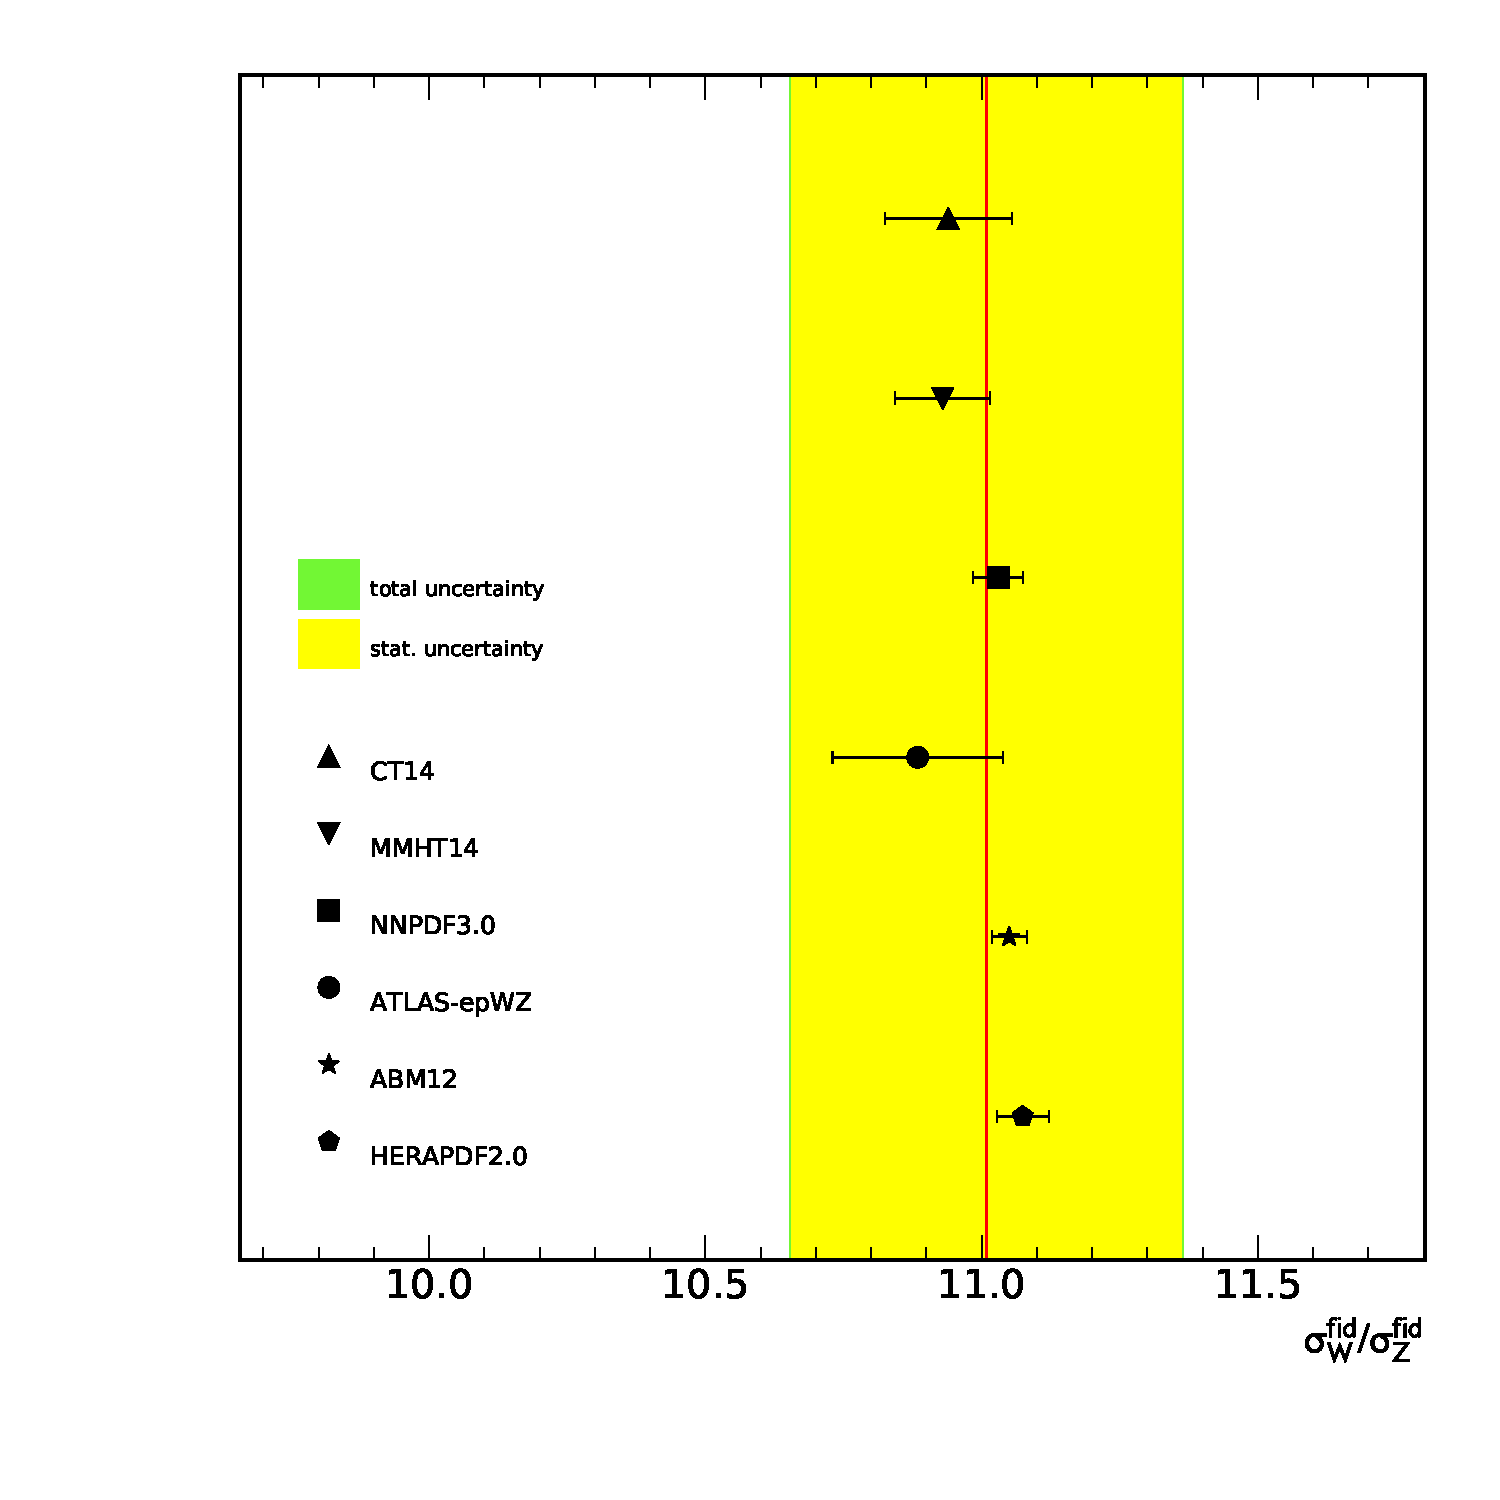
\includegraphics[width=1\textwidth]{Results/RatioWZ.pdf} \\ a)}
\end{minipage}
\hfill
\begin{minipage}[h]{0.49\linewidth}
\center{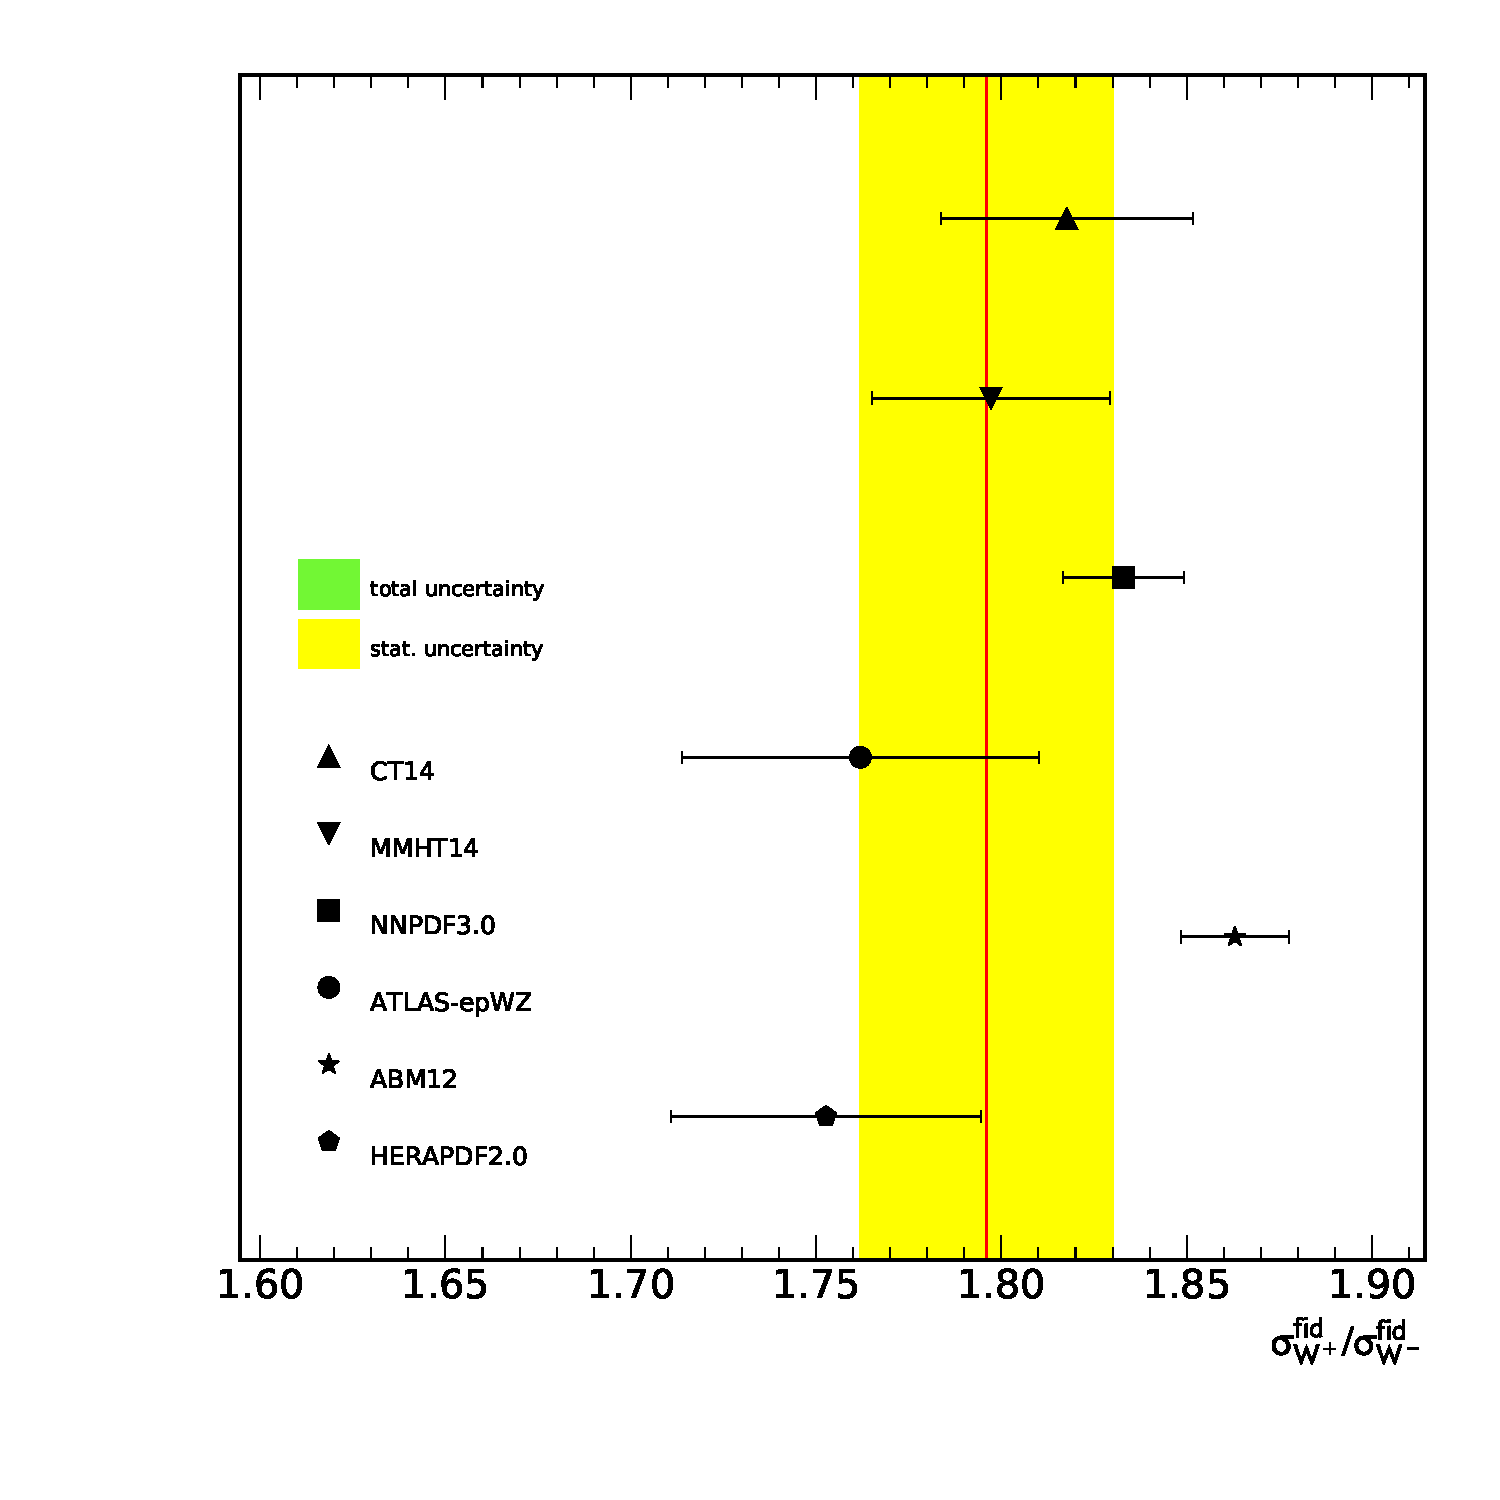
\includegraphics[width=1\textwidth]{Results/RatioWpWm.pdf}\\ b)}
\end{minipage}
\caption{Ratio of the a) W to Z  and b) $W^+$ to $W^-$ production fiducial cross-sections compared to predictions based on the six pdf sets:  CT14nnlo, MMHT2014, NNPDF3.0, ATLASepWZ12, abm12, HERApdf2.0. The yellow band corresponds to the statistical uncertainty, while the systematical uncertainty is considered to be negligible. The theory predictions are given with the corresponding PDF uncertainties shown as error bands.}
\label{fig:WRatio}
\end{figure}

\begin{figure}[!tbp]
\begin{minipage}[h]{0.49\linewidth}
\center{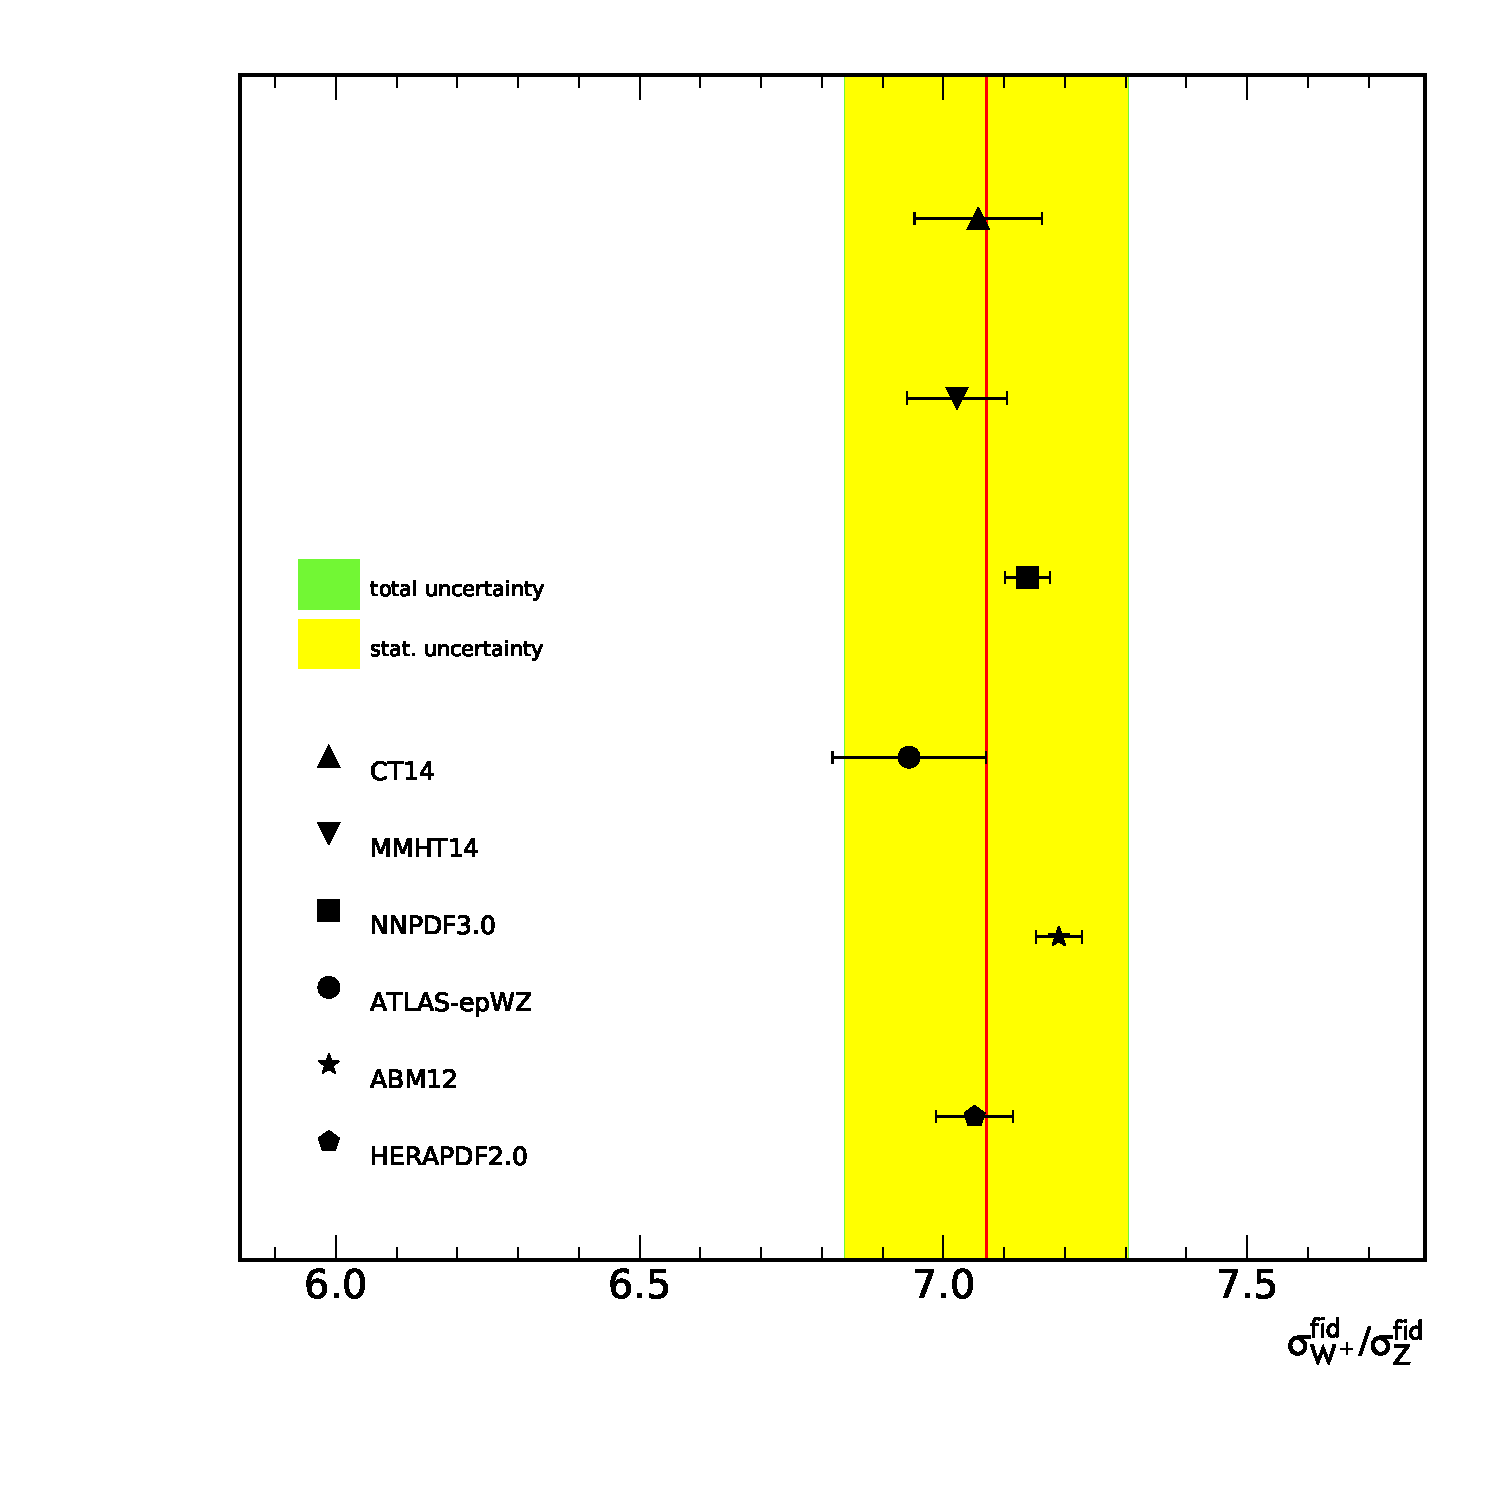
\includegraphics[width=1\textwidth]{Results/RatioWpZ.pdf} \\ a)}
\end{minipage}
\hfill
\begin{minipage}[h]{0.49\linewidth}
\center{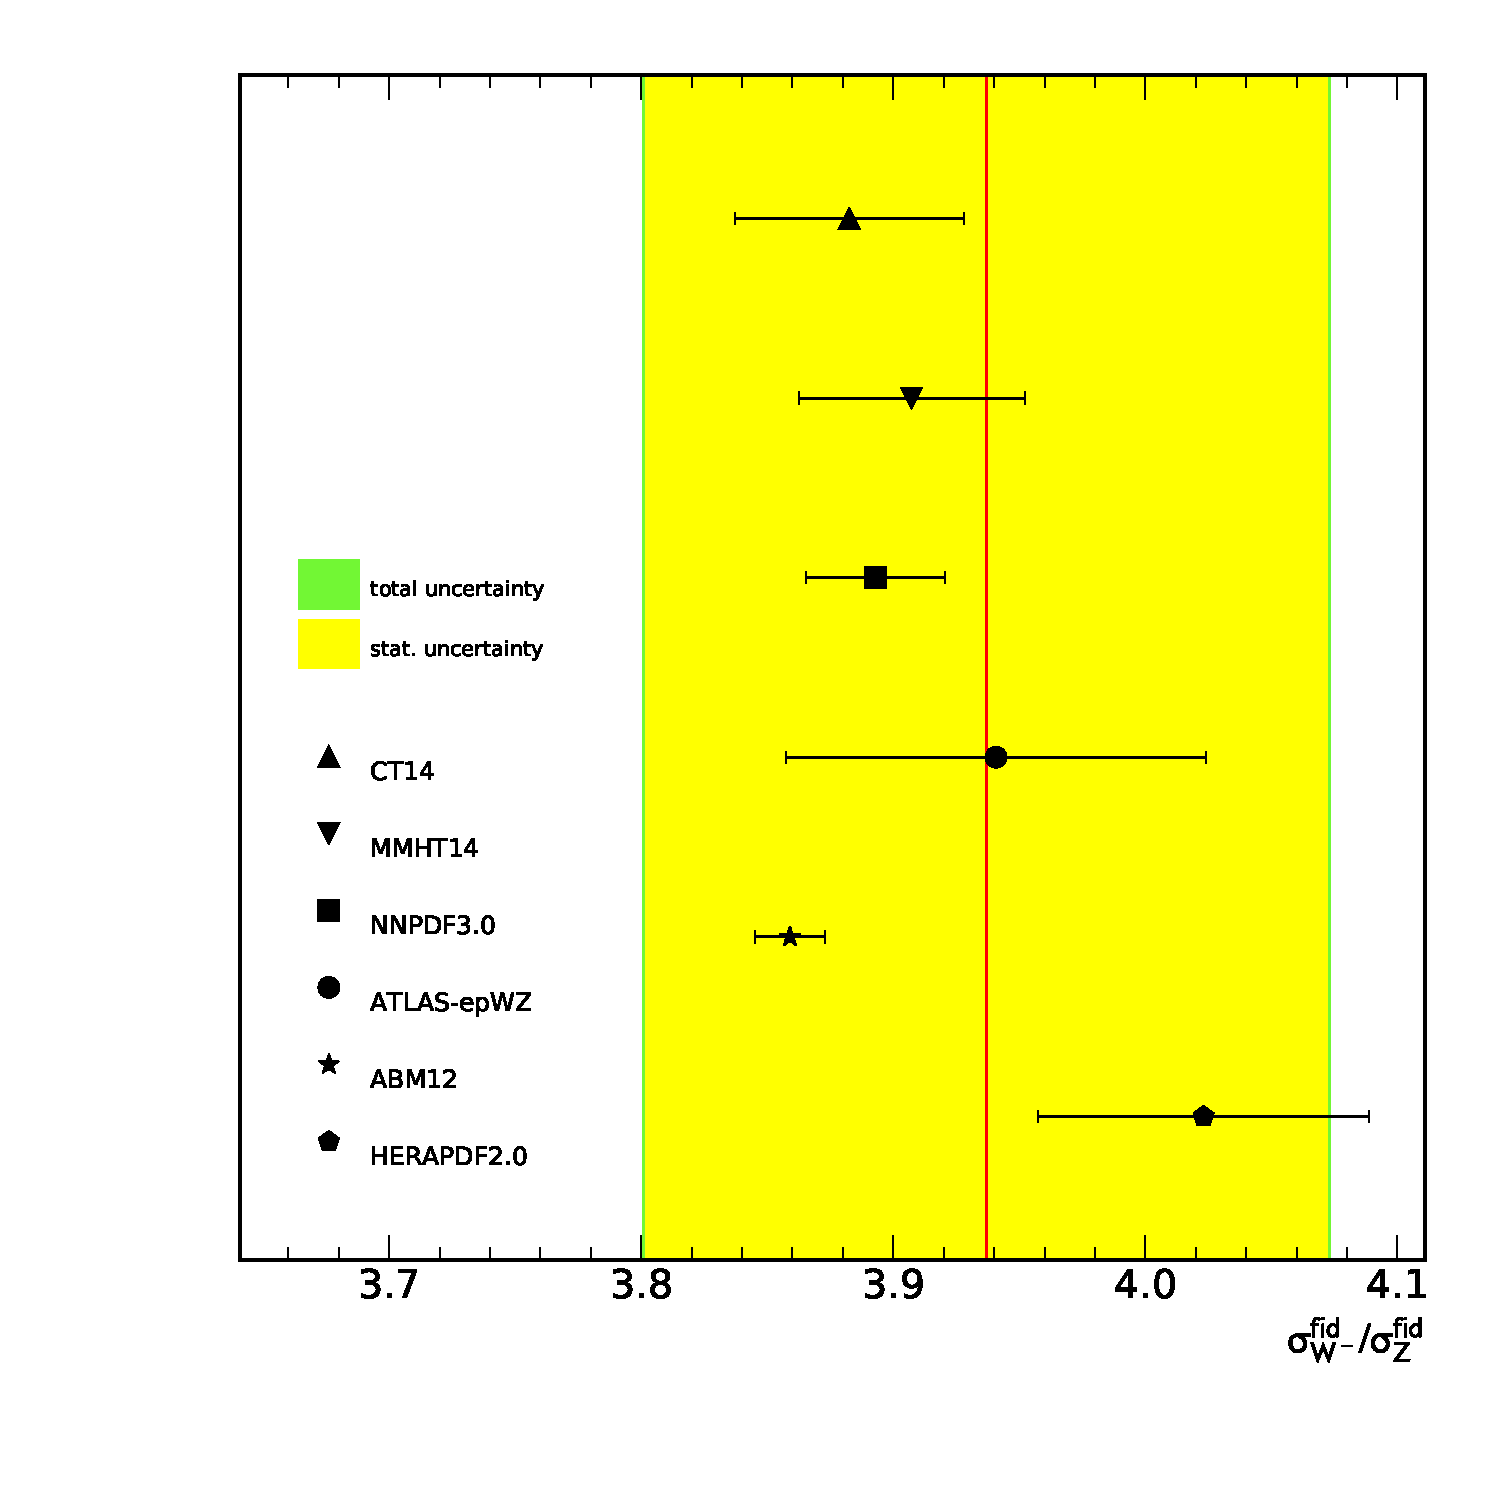
\includegraphics[width=1\textwidth]{Results/RatioWmZ.pdf} \\ b)}
\end{minipage}
\caption{Ratio of the a) $W^+$  to Z  and b) $W^-$ to Z production fiducial cross-sections compared to predictions based on the six pdf sets:  CT14nnlo, MMHT2014, NNPDF3.0, ATLASepWZ12, abm12, HERApdf2.0. The yellow band corresponds to the statistical uncertainty, while the systematical uncertainty is considered to be negligible. The theory predictions are given with the corresponding PDF uncertainties shown as error bands.}
\label{fig:ZRatio}
\end{figure}

\section{Effect on PDF distributions}\label{sec:PDFCs}

The effect of inclusion of obtained cross-sections in PDF set have been estimated using the profiling method, described in Sec.~\ref{sec:PDFFit}. As a reference, it was decided to use CT14 pdf set, because of its relatively good agreement with data for both NLO and NNLO predictions. The profiling was performed at NLO order, however it is also possible to make NNLO profiling with use of the NNLO K-factors.

As it was mentioned in Chap.~\ref{chap:Theory} the measurement at 2.76 TeV is mostly sensitive to the valence $u_v$ and $d_v$, light-sea $\bar{d}$ and $\bar{u}$ quark distributions. The inclusion of 2.76 TeV cross-sections in PDF can introduce both the reduction of the uncertainties of the PDF distributions and shift in the distributions. 

The sensitivity of this mesurement on the PDF uncertainties have been studied by adding in the PDF set the $W$ and $Z$ cross-sections scaled to match the theoretical predictions. This method does not introduce any shift in distributions, however, it makes a reduction of uncertainties more visible. The resulting distributions are shown in Fig.~\ref{fig:PDFSensitStrange} at the initial scale $Q^2=1.9$ GeV$^2$. This measurement allows to significantly reduce the uncertainties on $\bar{u}$ and $\bar{d}$ distributions. There is also a visible reduction of the uncertainties in the small x region for the valence quarks. Due to the limited statistics, the measurement can not reduce the uncertainties on the strange quark distributions. As it was expected, the $W$ and $Z$ cross-sections are not sensitive to the gluon density. It is possible to reduce the uncertainties on PDF distribution even more with inclusion of 5, 7 and 13 TeV $W$ and $Z$ cross-sections, because of the large number of correlated uncertainties for a different energy measurements (especially luminosity).

The full profiling results are shown in Fig.~\ref{fig:PDFValenceShift}-~\ref{fig:PDFSeaShift}. The initial value of $\chiD/NDF$=1.2/3 shows the good agreement with theoretical predictions, however the fit allows to reduce it to the down to the value $\chiD/NDF$=0.8/3. The profiling procedure introduces a shift in $u_v$, $d_v$, $\bar{u}$, $\bar{v}$, $s$ quark distributions within 1 sigma.  The gluon distribution is left untouched. The additional PDF profiling plots can be found in Appendix~\ref{app:PDF}.

The predictions of the obtained profiled CT14 set are shown in Fig.~\ref{fig:PDFEffectXsec}-~\ref{fig:PDFEffectRatio}. The cross-sections, predicted by the profiled CT14 set are in a better agreement, however not perfect, agreement with the data, compared to the original set. There is also a small reduction of the uncertainties.

\begin{figure}[!tbp]
\begin{minipage}[h]{0.43\linewidth}
\center{\includegraphics[width=1\textwidth]{Results/Sensitivity/uv_ratio.pdf} \\ a)}
\end{minipage}
\hfill
\begin{minipage}[h]{0.43\linewidth}
\center{\includegraphics[width=1\textwidth]{Results/Sensitivity/dv_ratio.pdf} \\ b)}
\end{minipage}
\vfill
\begin{minipage}[h]{0.43\linewidth}
\center{\includegraphics[width=1\textwidth]{Results/Sensitivity/UBar_ratio.pdf} \\ c)}
\end{minipage}
\hfill
\begin{minipage}[h]{0.43\linewidth}
\center{\includegraphics[width=1\textwidth]{Results/Sensitivity/DBar_ratio.pdf} \\ d)}
\end{minipage}
\vfill
\begin{minipage}[h]{0.43\linewidth}
\center{\includegraphics[width=1\textwidth]{Results/Sensitivity/s_ratio.pdf} \\ e)}
\end{minipage}
\hfill
\begin{minipage}[h]{0.43\linewidth}
\center{\includegraphics[width=1\textwidth]{Results/Sensitivity/g_ratio.pdf} \\ f)}
\end{minipage}
\caption{The relative experimental uncertainties for the quark and gluon densities as a function of $x$ at scale $Q^2=$ 1.9 GeV$^2$. The red band denotes the reference NLO PDF distributions from CT14 pdf set. The impact of addition of the new W,Z cross-sections at 2.76 TeV on the PDF set uncertainties is shown by the blue boundaries.}
\label{fig:PDFSensitStrange}
\end{figure}

\begin{figure}[!tbp]
\begin{minipage}[h]{0.43\linewidth}
\center{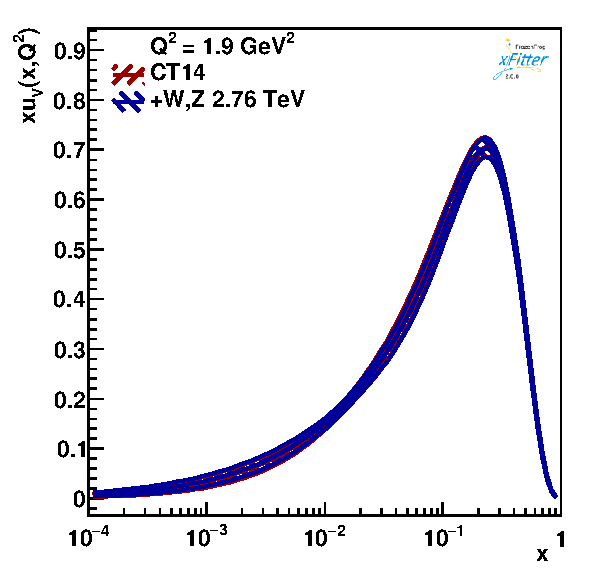
\includegraphics[width=1\textwidth]{Results/Shift/uv.pdf} \\ a)}
\end{minipage}
\hfill
\begin{minipage}[h]{0.43\linewidth}
\center{\includegraphics[width=1\textwidth]{Results/Shift/uv_ratio.pdf} \\ b)}
\end{minipage}
\vfill
\begin{minipage}[h]{0.43\linewidth}
\center{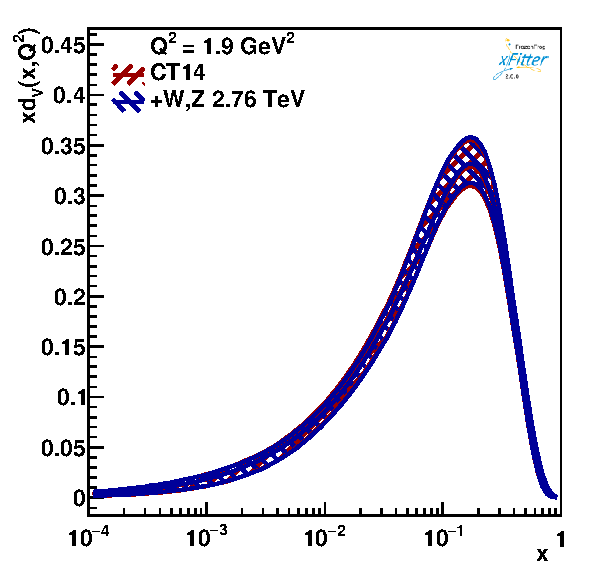
\includegraphics[width=1\textwidth]{Results/Shift/dv.pdf} \\ c)}
\end{minipage}
\hfill
\begin{minipage}[h]{0.43\linewidth}
\center{\includegraphics[width=1\textwidth]{Results/Shift/dv_ratio.pdf} \\ d)}
\end{minipage}
\vfill
\begin{minipage}[h]{0.43\linewidth}
\center{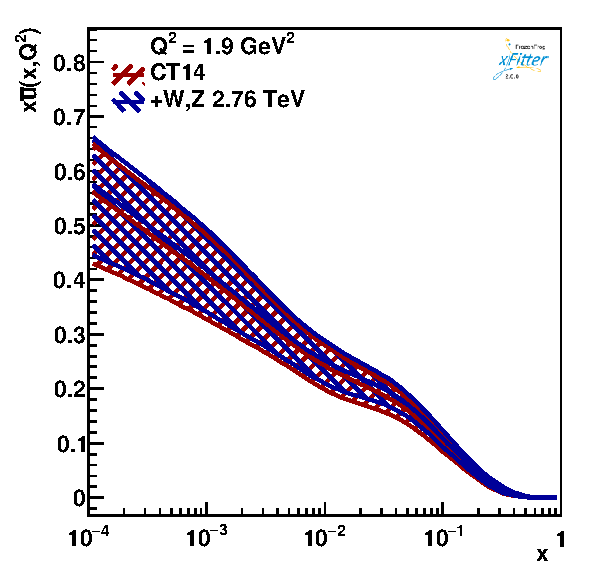
\includegraphics[width=1\textwidth]{Results/Shift/UBar.pdf} \\ e)}
\end{minipage}
\hfill
\begin{minipage}[h]{0.43\linewidth}
\center{\includegraphics[width=1\textwidth]{Results/Shift/UBar_ratio.pdf} \\ f)}
\end{minipage}
\caption{The absolute and  relative distributions for the $u_v$, $d_v$, $\bar{u}$ quark densities as a function of $x$ at scale $Q^2=$ 1.9 GeV$^2$ with the experimental uncertainties. The red band denotes the reference NLO PDF distributions from CT14 pdf set. The impact of addition of the new W,Z cross-sections at 2.76 TeV on the PDF set is shown by the blue boundaries.}
\label{fig:PDFValenceShift}
\end{figure}

\begin{figure}[!tbp]
\begin{minipage}[h]{0.43\linewidth}
\center{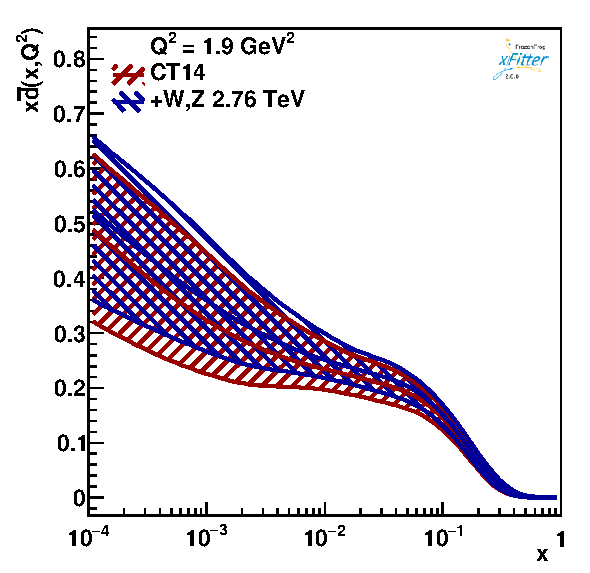
\includegraphics[width=1\textwidth]{Results/Shift/DBar.pdf} \\ a)}
\end{minipage}
\hfill
\begin{minipage}[h]{0.43\linewidth}
\center{\includegraphics[width=1\textwidth]{Results/Shift/DBar_ratio.pdf} \\ b)}
\end{minipage}
\vfill
\begin{minipage}[h]{0.43\linewidth}
\center{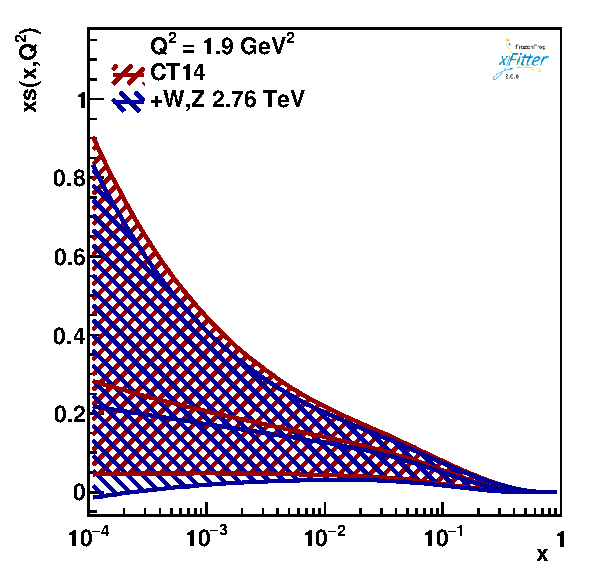
\includegraphics[width=1\textwidth]{Results/Shift/s.pdf} \\ c)}
\end{minipage}
\hfill
\begin{minipage}[h]{0.43\linewidth}
\center{\includegraphics[width=1\textwidth]{Results/Shift/s_ratio.pdf} \\ d)}
\end{minipage}
\vfill
\begin{minipage}[h]{0.43\linewidth}
\center{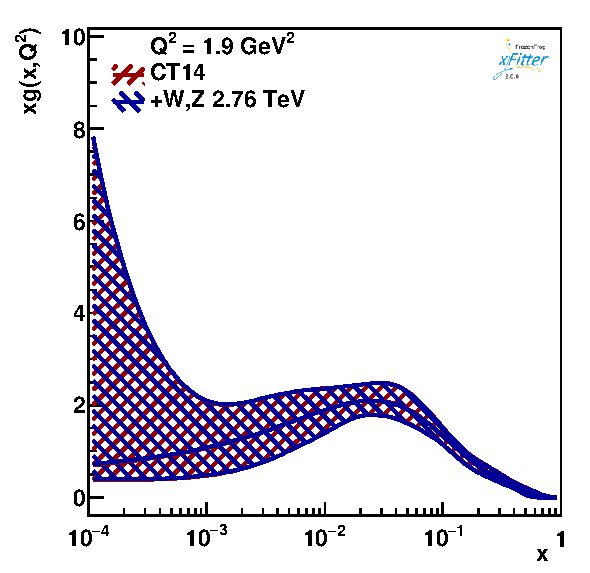
\includegraphics[width=1\textwidth]{Results/Shift/g.pdf} \\ e)}
\end{minipage}
\hfill
\begin{minipage}[h]{0.43\linewidth}
\center{\includegraphics[width=1\textwidth]{Results/Shift/g_ratio.pdf} \\ f)}
\end{minipage}
\caption{The absolute and  relative distributions for the $\bar{d}$ and $s$ quark and gluon densities as a function of $x$ at scale $Q^2=$ 1.9 GeV$^2$ with the experimental uncertainties. The red band denotes the reference NLO PDF distributions from CT14 pdf set. The impact of addition of the new W,Z cross-sections at 2.76 TeV on the PDF set is shown by the blue boundaries.}
\label{fig:PDFSeaShift}
\end{figure}


%\begin{figure}[!tbp]
%\begin{center}
%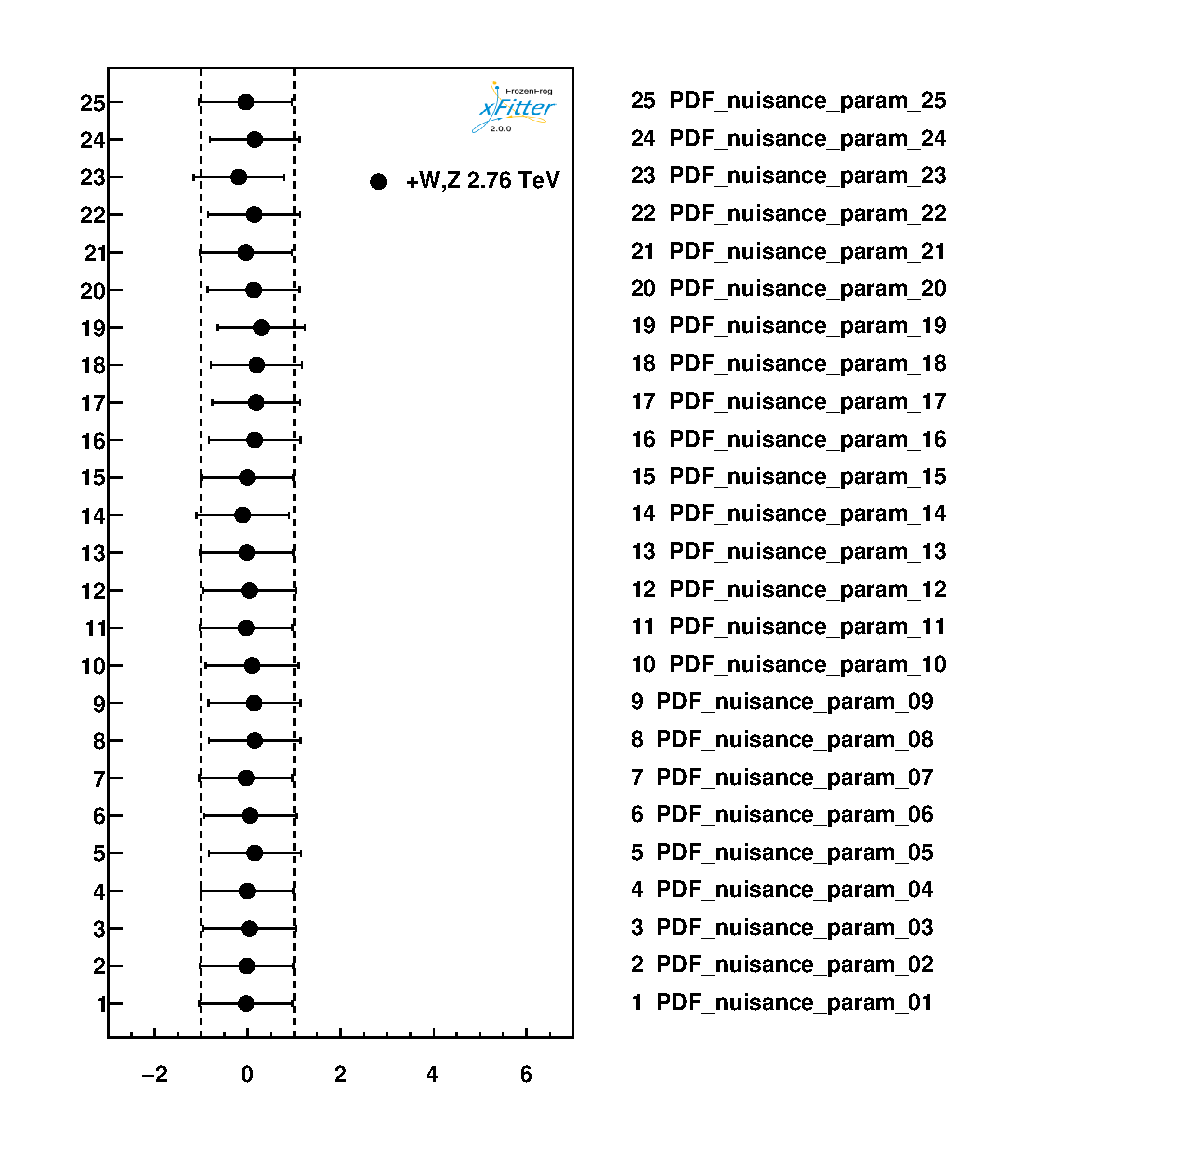
\includegraphics[width=0.7\textwidth]{Results/shifts_0.pdf}
%\end{center}
%\caption{Relative shift in PDF nuisance parameters due to the PDF profiling}
%\label{fig:shiftPDF}
%\end{figure}

\begin{figure}[!tbp]
\begin{minipage}[h]{0.32\linewidth}
\center{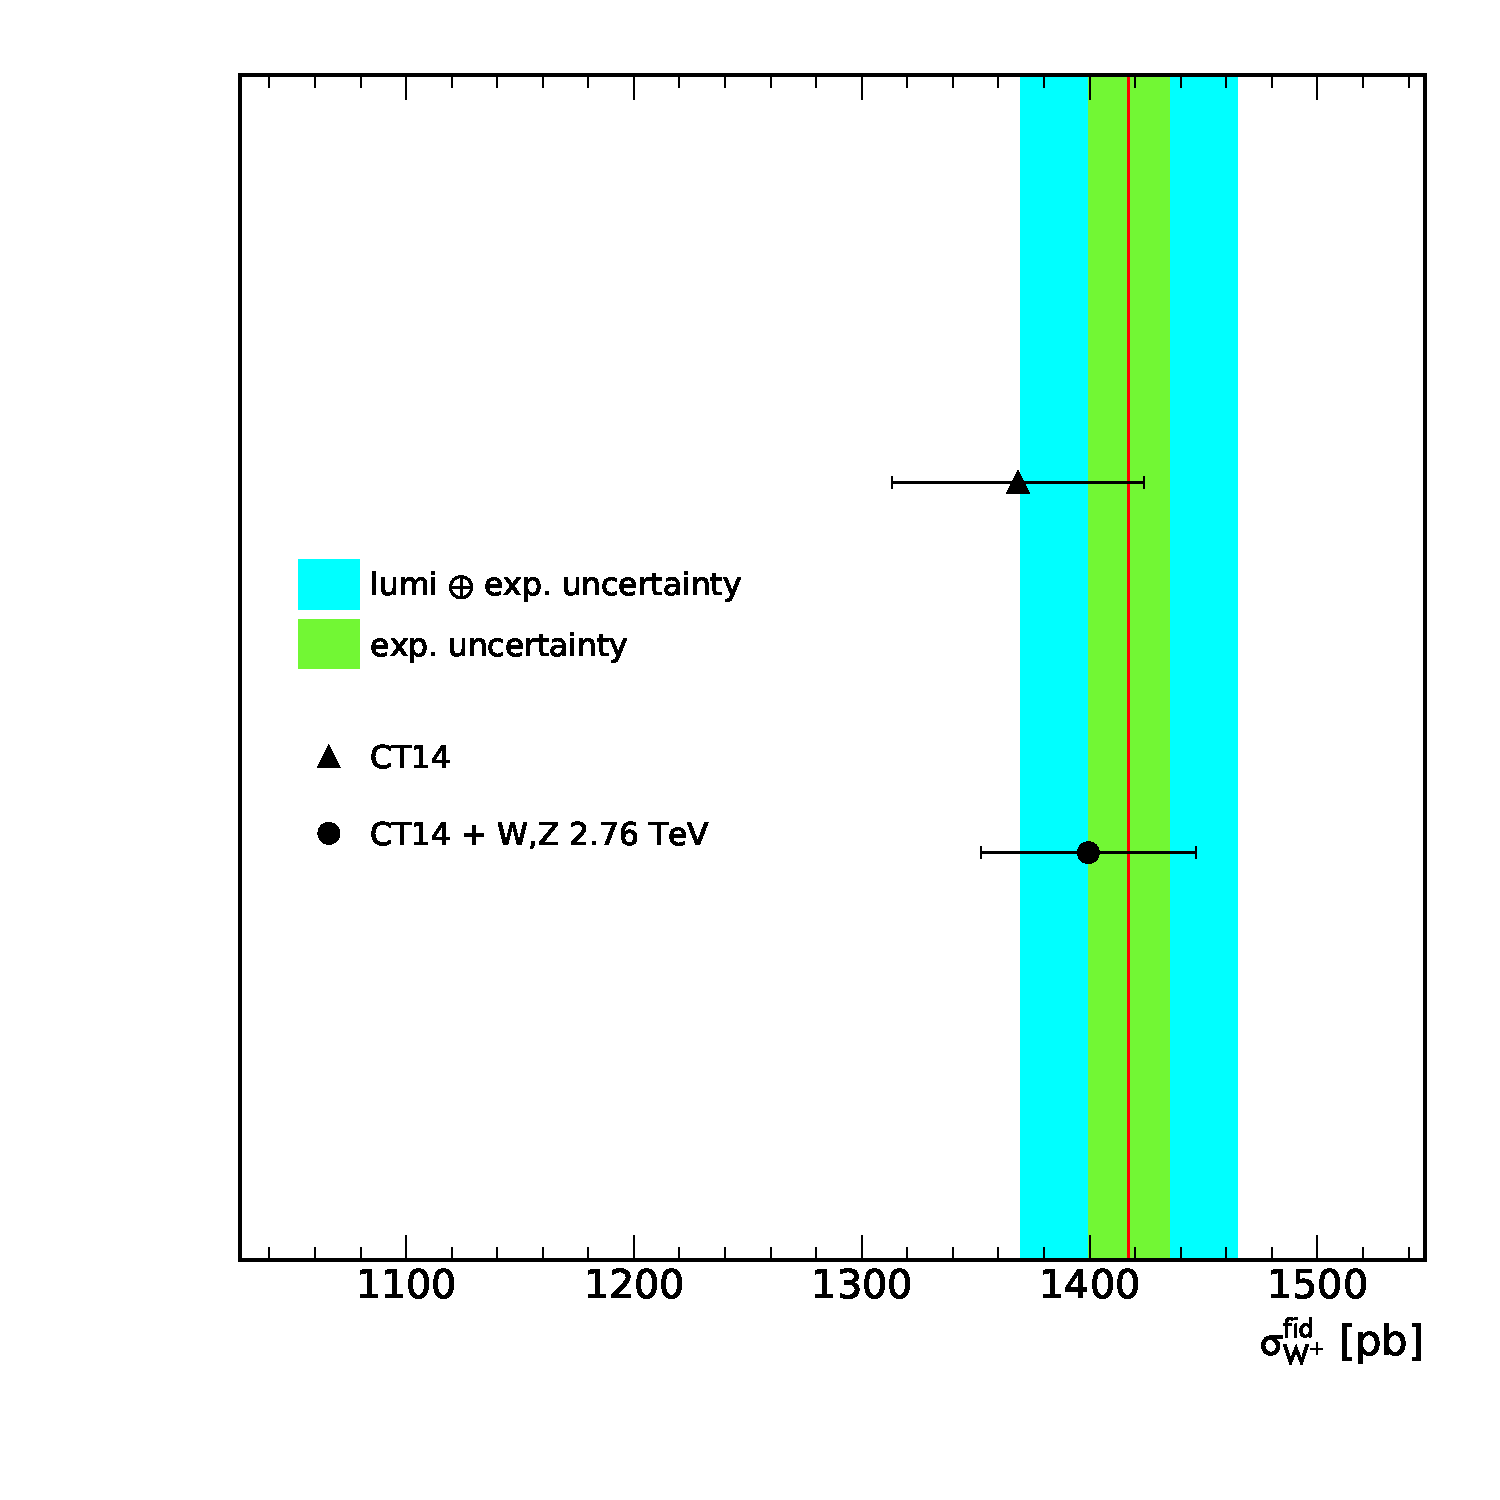
\includegraphics[width=1\textwidth]{Results/PDFImpWPlus.pdf} \\ a)}
\end{minipage}
\hfill
\begin{minipage}[h]{0.32\linewidth}
\center{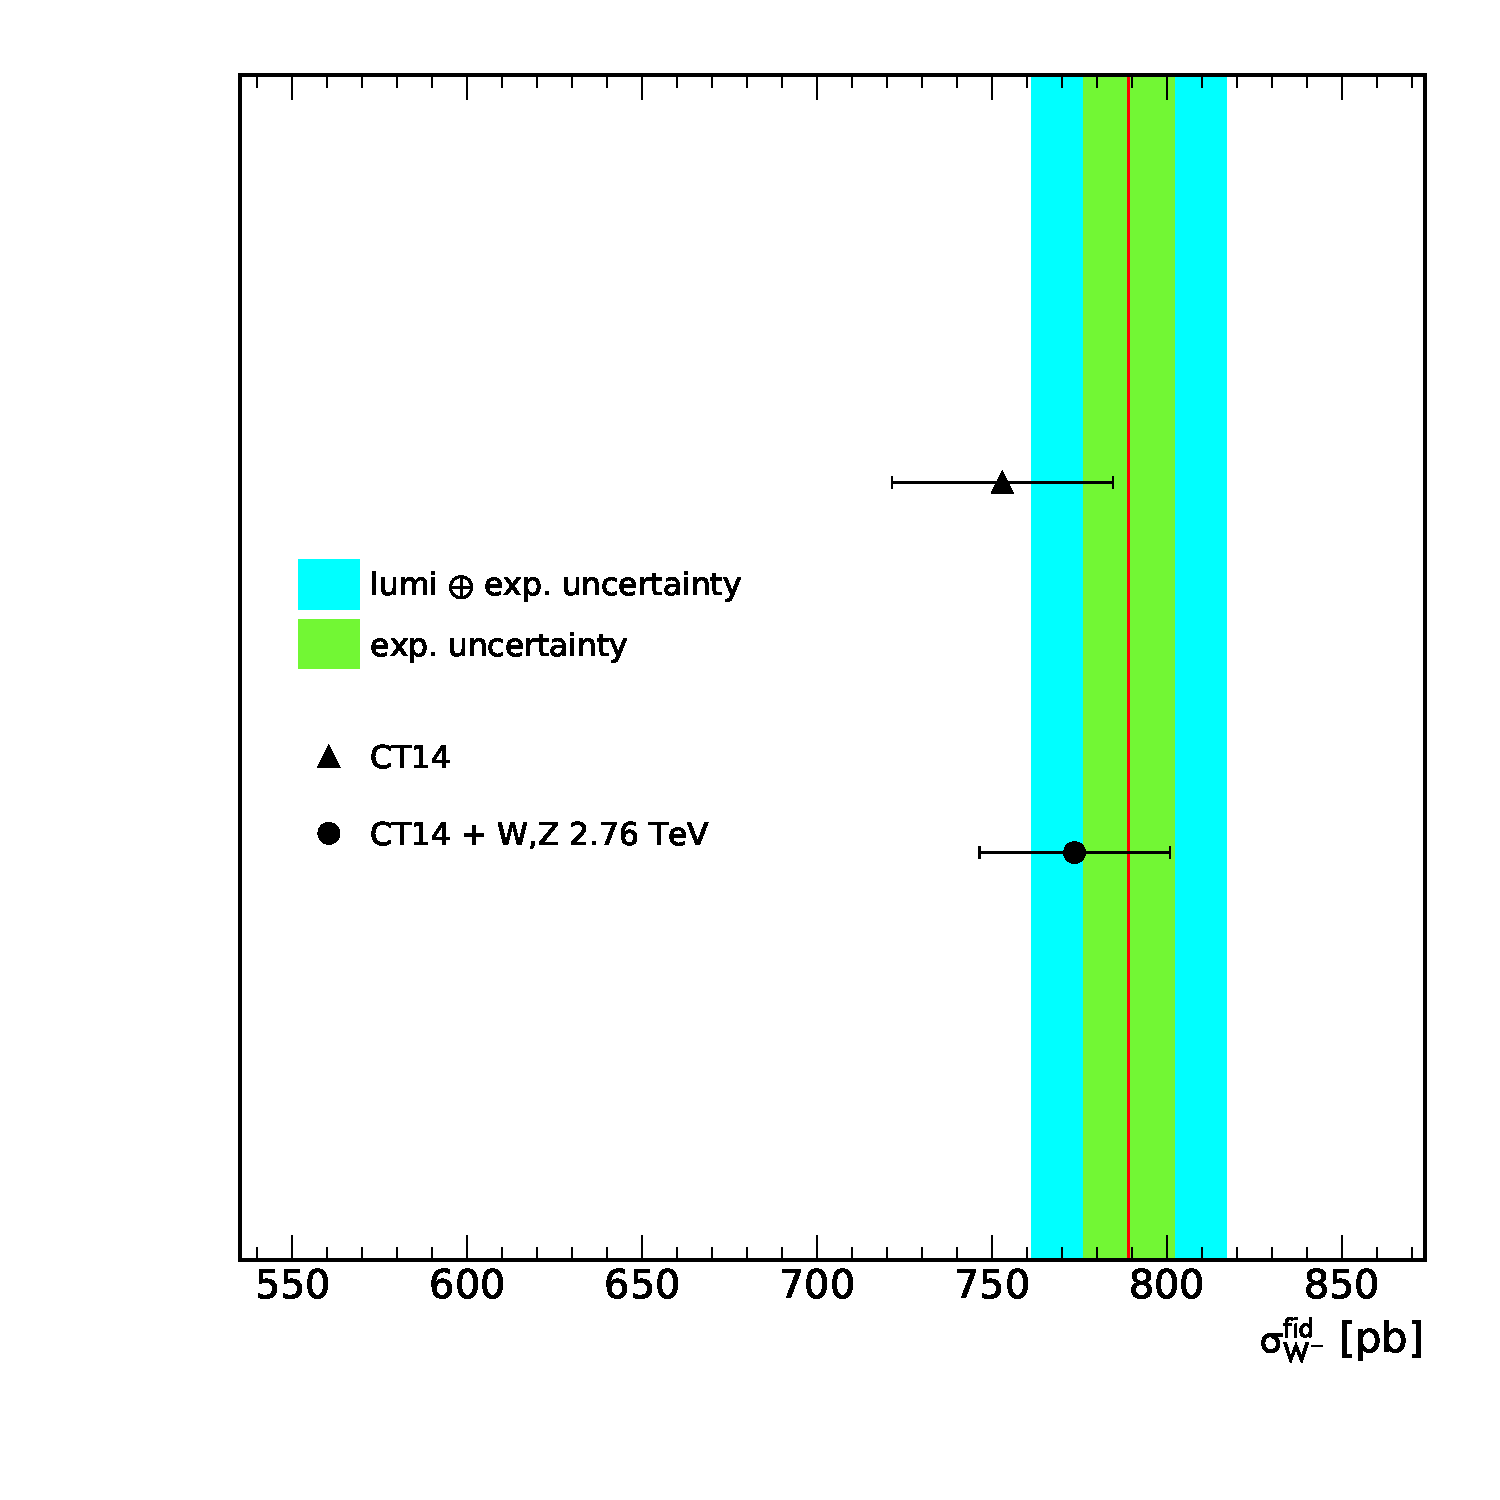
\includegraphics[width=1\textwidth]{Results/PDFImpWMinus.pdf} \\ b)}
\end{minipage}
\hfill
\begin{minipage}[h]{0.32\linewidth}
\center{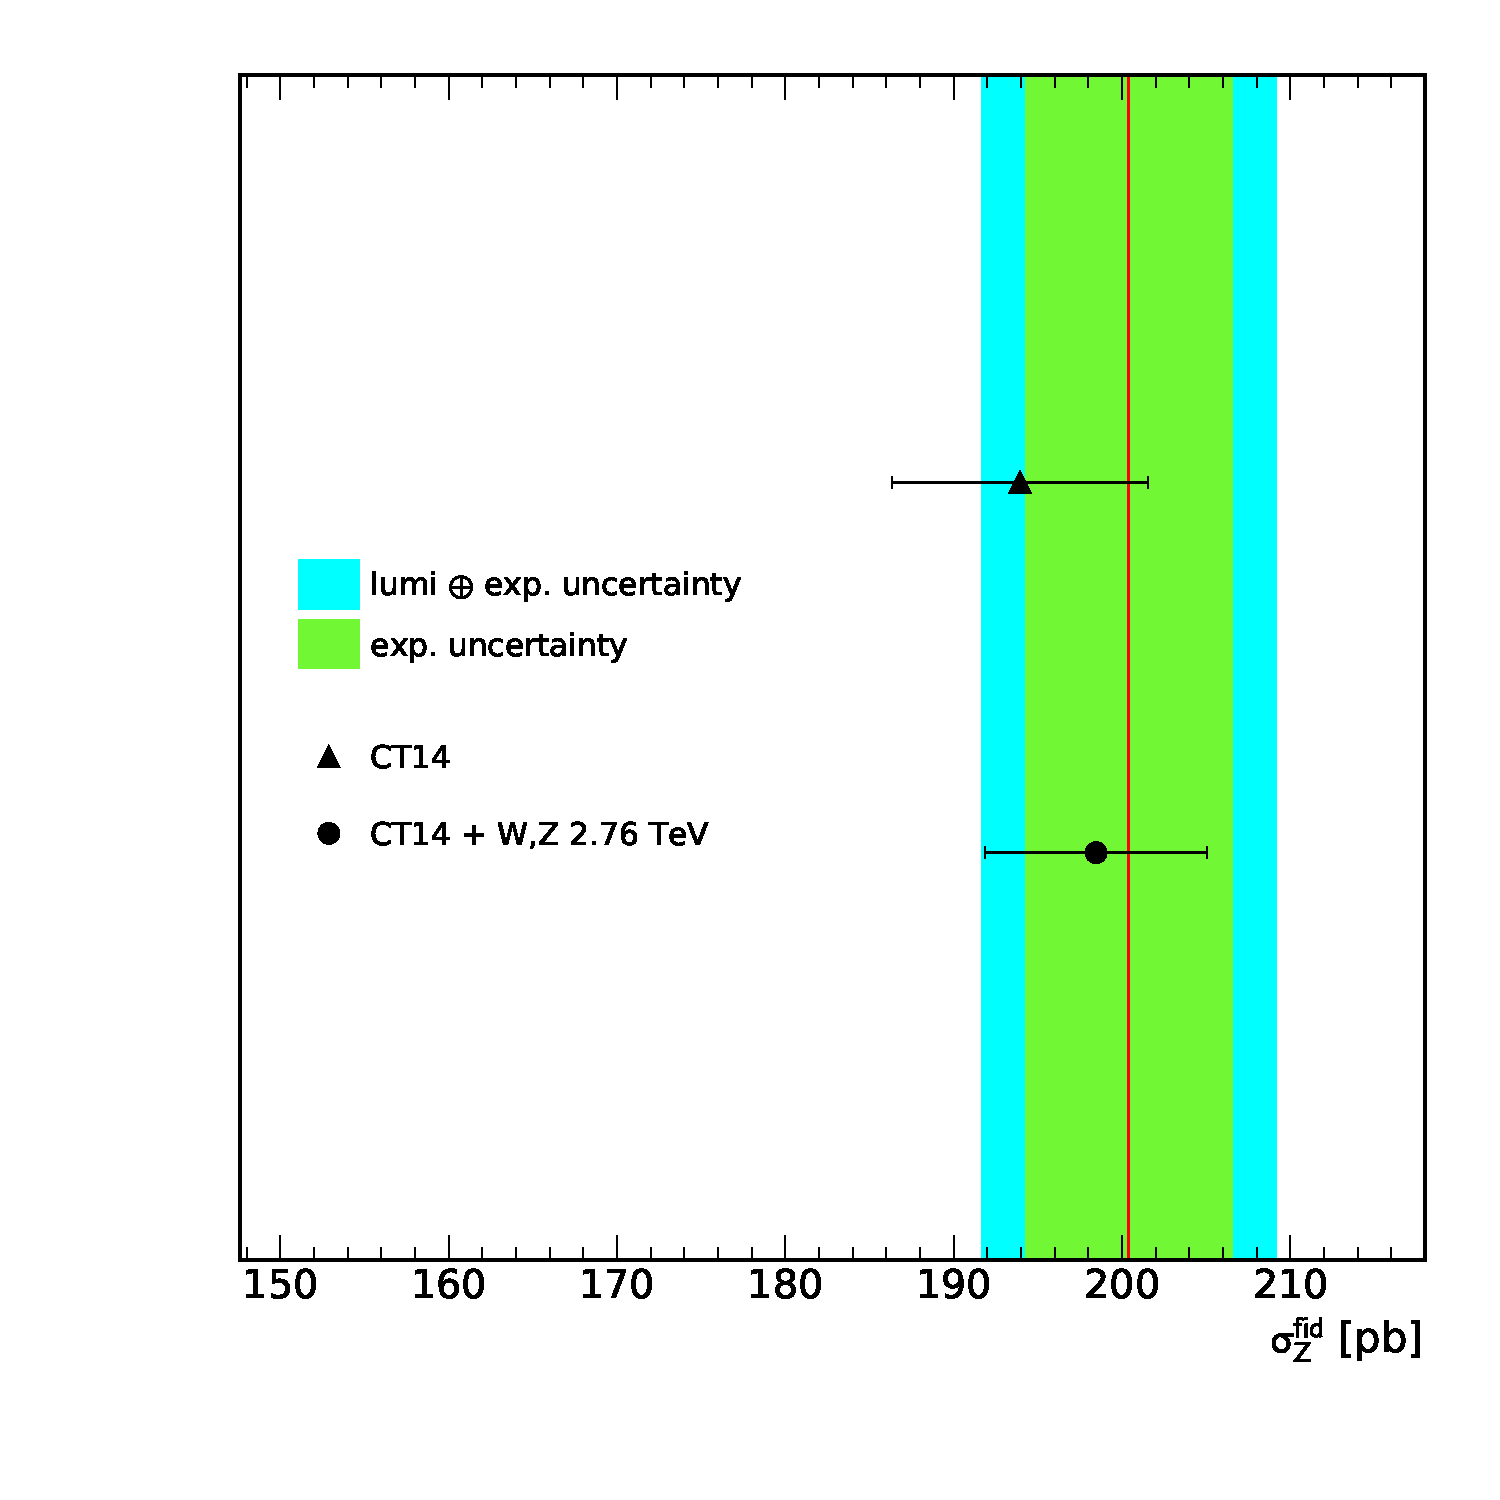
\includegraphics[width=1\textwidth]{Results/PDFImpZ.pdf} \\ c)}
\end{minipage}
\caption{The obtained a) $W^{+}$  b) $W^-$  c) $Z$ production fiducial cross-sections in combined channel compared to NLO predictions based on original and profiled CT14 PDF set.}
\label{fig:PDFEffectXsec}
\end{figure}



\begin{figure}[!tbp]
\begin{minipage}[h]{0.49\linewidth}
\center{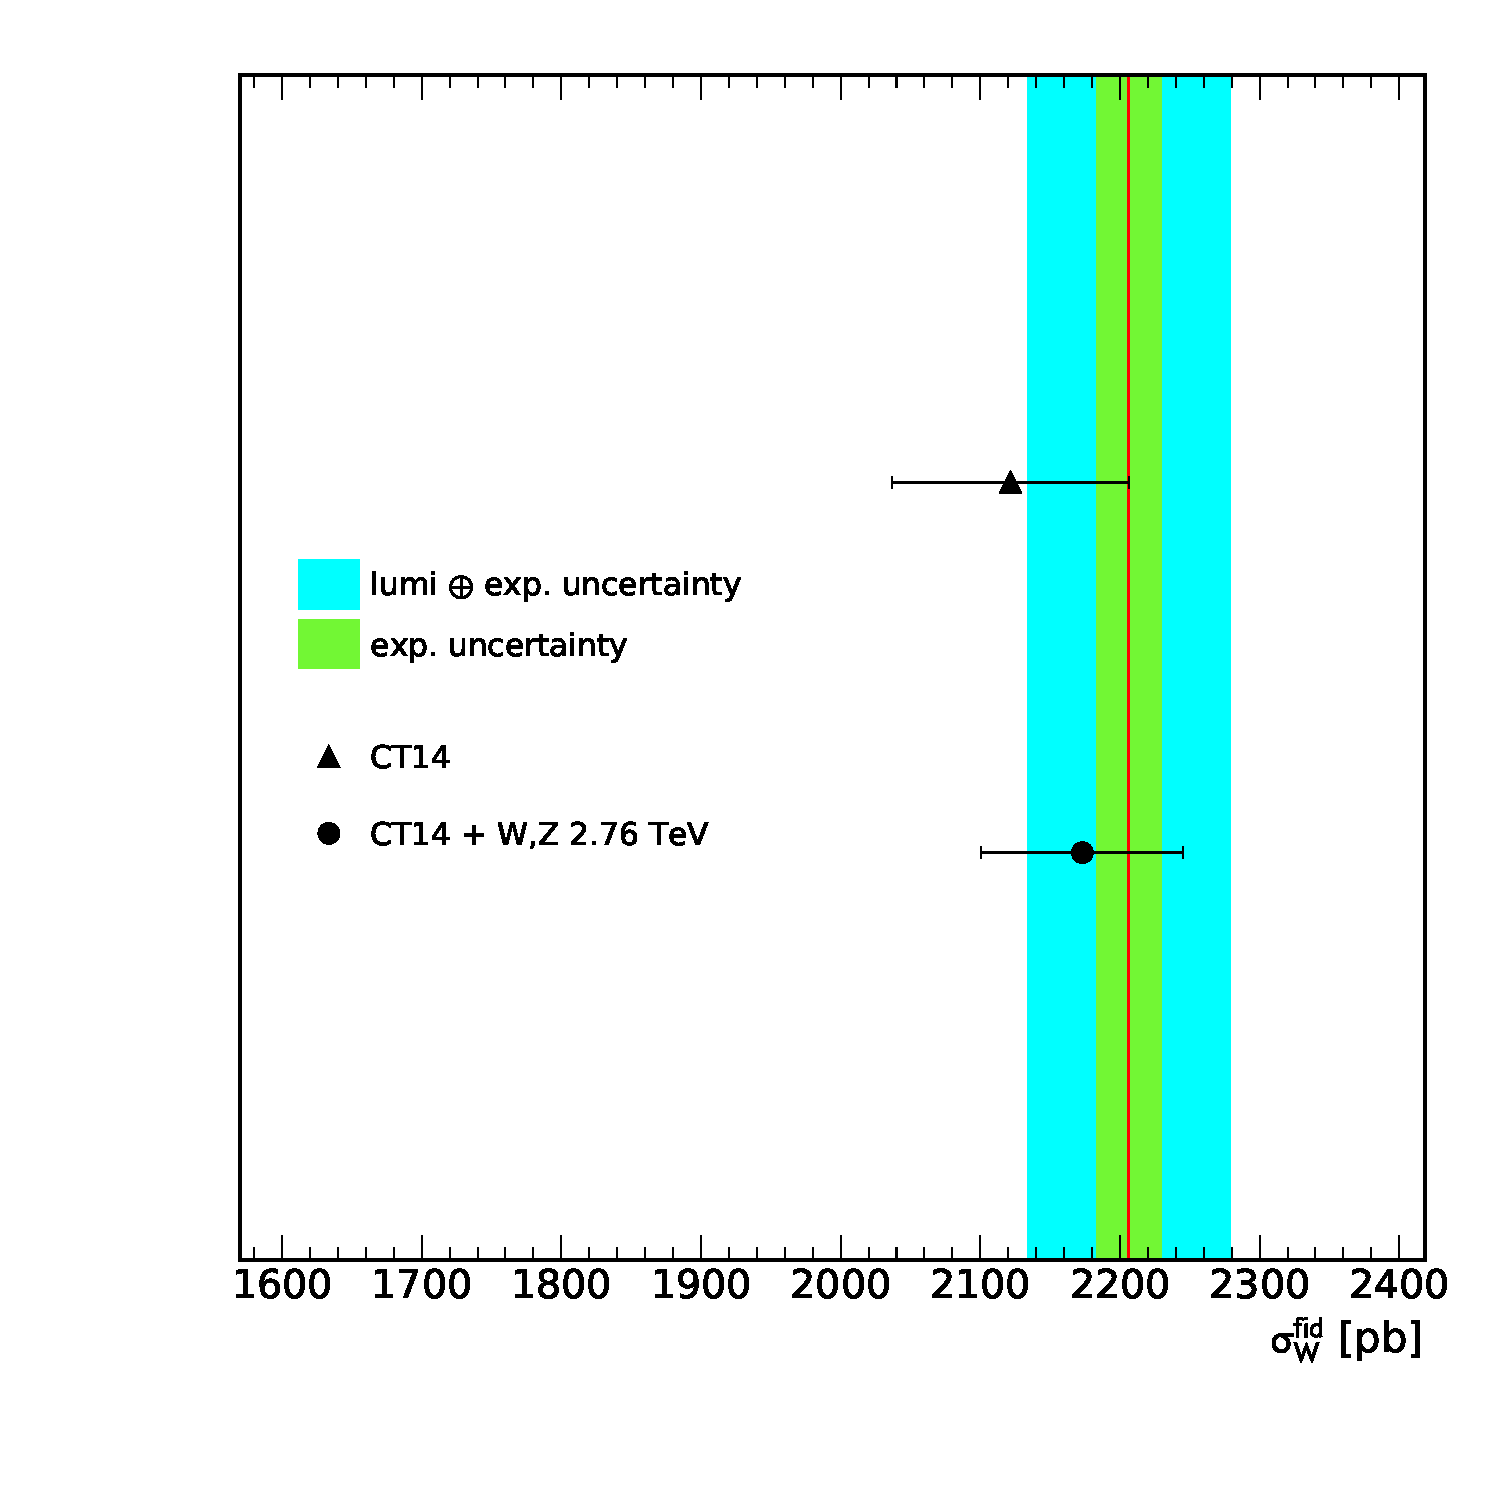
\includegraphics[width=1\textwidth]{Results/PDFImpW.pdf} \\ c)}
\end{minipage}
\begin{minipage}[h]{0.49\linewidth}
\center{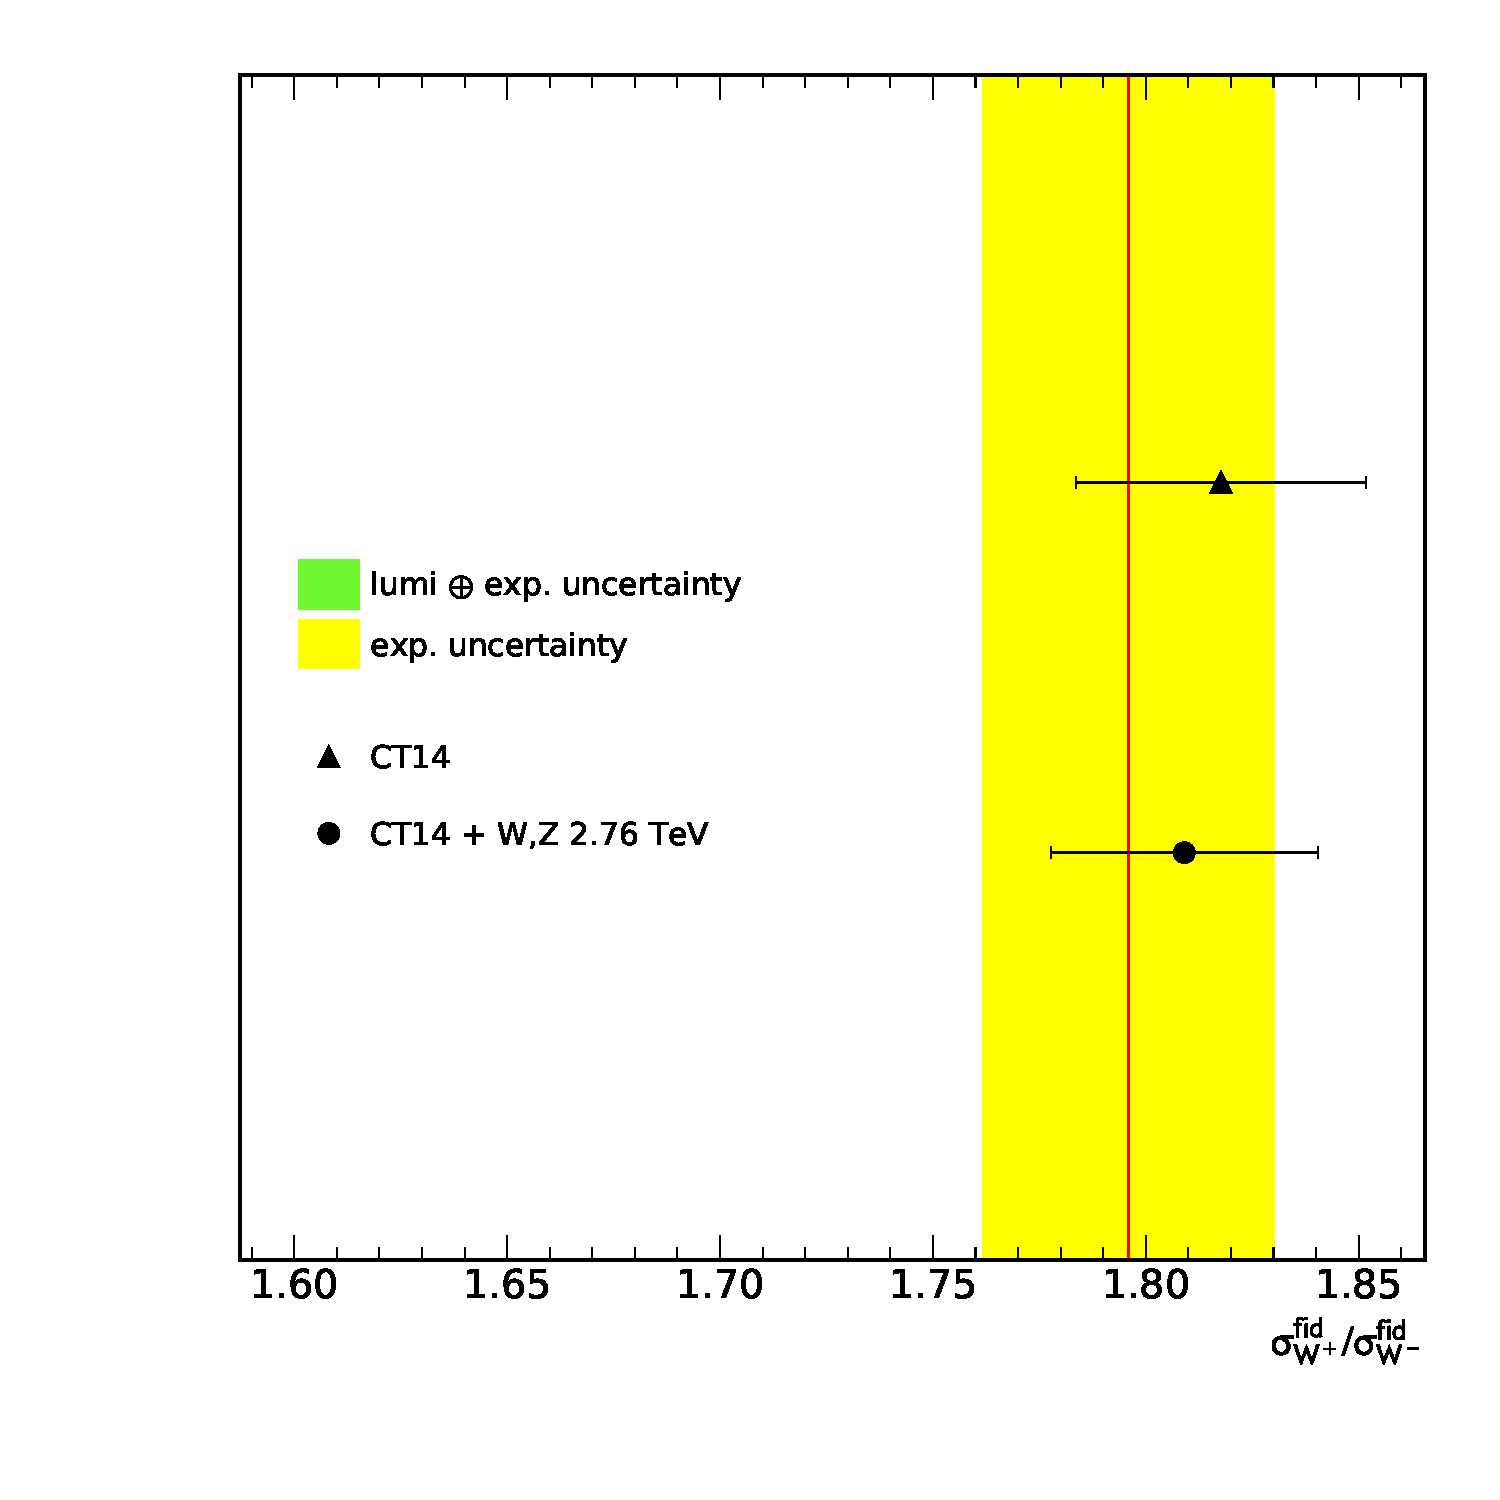
\includegraphics[width=1\textwidth]{Results/PDFImpRatioWpWm.pdf} \\ b)}
\end{minipage}
\caption{The obtained a)$W$  and  b) ratio of the  $W^+$ to $W^-$ production fiducial cross-sections in combined channel compared to NLO predictions based on original and profiled CT14 PDF set. }
\label{fig:PDFEffectRatio}
\end{figure}
